\section{Resultados e Discussão}
\subsection{Organização da matriz de resultados}
Os 17 compostos selecionados para prospecção reúnem monossacarídeos, derivados de açúcares e fenólicos descritos em estudos sobre SPE e outros materiais microalgais. O Quadro~\ref{quad:ligantes_spe_literatura} especifica o material e a espécie associados às evidências de ocorrência de cada composto.

A matriz reúne 204 combinações de 34 ligantes com seis receptores humanos, cada uma representada pela menor FEB entre as poses disponíveis. As execuções com coordenadas corrigidas de 1H1B e 2PE4 atualizaram 68 resultados: 17 ligantes comerciais e coocristalizados e 17 compostos selecionados para prospecção em cada receptor. Para os outros quatro receptores, foram mantidos os resultados anteriores. A Tabela~\ref{tab:melhores} compara as menores FEB dos dois conjuntos em cada alvo. Em todos os receptores, a menor FEB dos ligantes comerciais e coocristalizados foi mais negativa que a dos compostos em prospecção; esses valores destacam as poses mais bem avaliadas pela função adotada.

\begin{table}[H]
\centering\caption[Menores pontuações por conjunto]{Menores pontuações de docking (FEB, kcal/mol) dos ligantes comerciais e coocristalizados e dos compostos selecionados para prospecção nos seis receptores humanos.}\label{tab:melhores}
\begin{tabular}{C{1.2cm}C{3.3cm}C{1.9cm}C{3.7cm}C{1.9cm}}
\toprule PDB & Ligantes comerciais e coocristalizados & FEB (kcal/mol) & Compostos em prospecção & FEB (kcal/mol) \\\midrule
1GKC & L2U & -13,465 & Glicose-6-sulfato & -6,971 \\
1HFC & GW475151 & -12,366 & Glicose-6-sulfato & -7,591 \\
8H78 & L2U & -15,656 & Galactose-6-sulfato & -6,802 \\
5M8P & Batimastat & -9,216 & Ácido ferúlico & -6,020 \\
1H1B & ARP-100 & -6,535 & Dha & -5,359 \\
2PE4 & Cromoglicato & -9,199 & Dha & -6,033 \\
\bottomrule\end{tabular}
\end{table}

Em 5M8P, a L-tirosina apresentou FEB de -10,103~kcal/mol em uma análise suplementar, fora do conjunto principal de 34 ligantes. O batimastat, com -9,216~kcal/mol, ocupou a primeira posição entre os ligantes comerciais e coocristalizados. A L-tirosina é uma referência estrutural para a análise de sobreposição e não foi adotada como controle positivo de inibição.

\subsection{RMSD e comparação com as referências cristalográficas}
A Tabela~\ref{tab:rmsd_fit} apresenta as poses selecionadas pelo menor RMSD após ajuste independente, critério distinto da menor FEB. Esse ajuste compara as conformações das moléculas depois do alinhamento.

\begin{table}[H]
\centering\caption[Menores RMSD após sobreposição]{Menores RMSD após sobreposição independente dos ligantes.}\label{tab:rmsd_fit}
\begin{tabular}{C{1.5cm}C{4.8cm}C{2.0cm}C{2.0cm}}
\toprule PDB & Ligante & Pose & RMSD (\AA) \\\midrule
1GKC & NFH & 01 & 1,302 \\
1HFC & PLH & 01 & 1,074 \\
5M8P & L-tirosina & 03 & 0,261 \\
8H78 & L2U & 04 & 3,451 \\
1H1B & GW475151 & 03 & 1,836 \\
\bottomrule\end{tabular}
\fonte{Análise consolidada de sobreposição conformacional dos ligantes.}
\end{table}

Os resultados de sobreposição conformacional foram preservados como análise da execução anterior e não foram recalculados para as novas poses de 1H1B e 2PE4. Portanto, a pose 03 e o RMSD de GW475151 nessa análise não devem ser atribuídos à execução com coordenadas corrigidas. Em 1H1B, a comparação parcial (29/30 átomos, O51 ausente na referência covalente) limita a interpretação; 2PE4 não possui referência equivalente. O limiar de 2~\AA{} não assegura validação universal \parencite{cole2005,macdonald2002}. As Figuras~\ref{fig:fit_1GKC}, \ref{fig:fit_1HFC}, \ref{fig:fit_5M8P}, \ref{fig:fit_8H78} e~\ref{fig:fit_1H1B} mostram as sobreposições avaliadas, na mesma ordem da Tabela~\ref{tab:rmsd_fit}. Cada figura é seguida pelos contatos da pose correspondente; as legendas identificam os tipos de interação. As coordenações exclusivamente metal--receptor não entram nas contagens ligante--aminoácido.

\begin{figure}[H]\centering
\centering
\caption[Sobreposição de NFH em 1GKC]{Sobreposição de NFH com sua referência cristalográfica em 1GKC: pose 01, RMSD de 1,302~\AA.}\label{fig:fit_1GKC}
\par\centering\normalsize\begin{tabular}{@{}l@{\hspace{1.5em}}l@{}}\tikz[baseline=-.4ex]\filldraw[fill=orange,draw=black!40] (0,0) rectangle (.28,.28);\ Ligante dockado & \tikz[baseline=-.4ex]\filldraw[fill=forestgreen,draw=black!40] (0,0) rectangle (.28,.28);\ Ligante cristalográfico\end{tabular}\par\vspace{3pt}
\begin{tikzpicture}
\node[inner sep=0] (molecula) {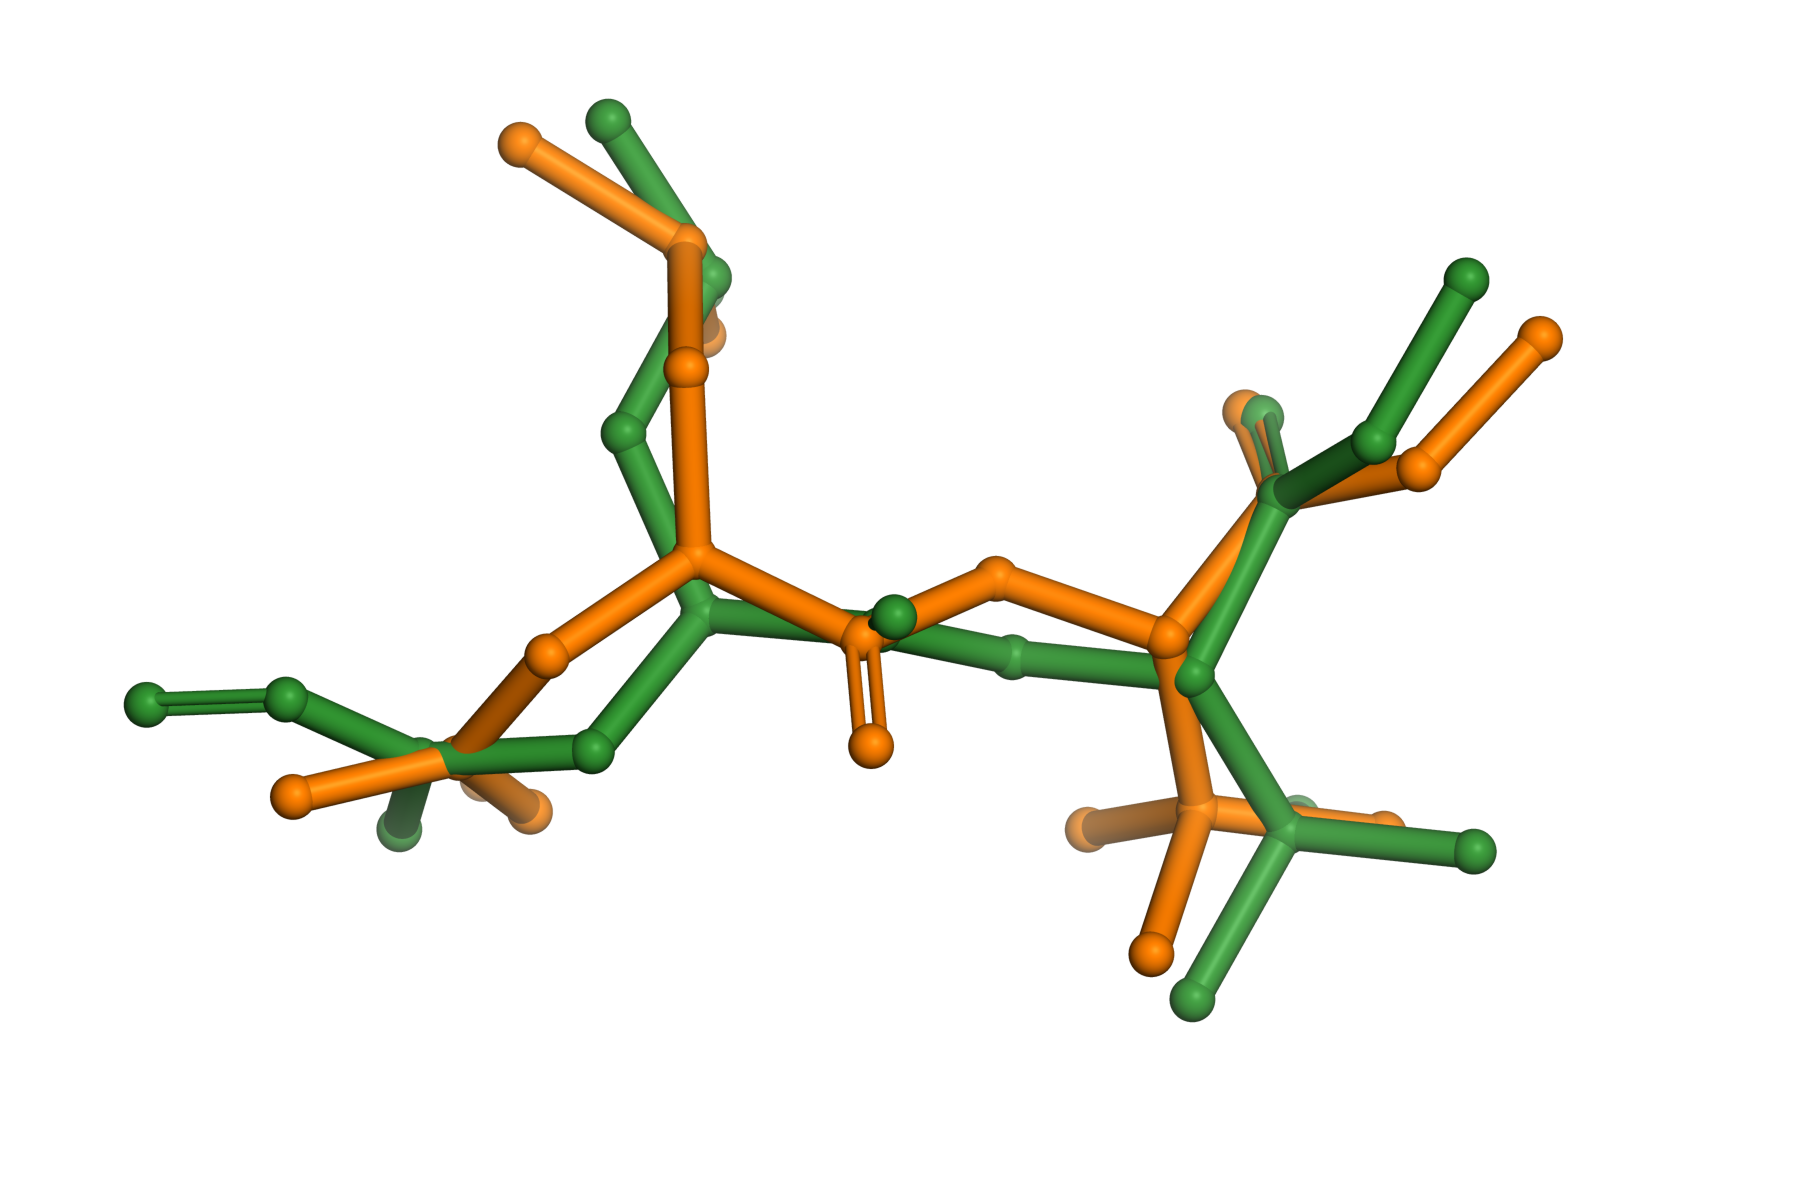
\includegraphics[width=.65\linewidth]{image/sobreposicoes_ligantes/1GKC_ligantes_sobrepostos.png}};
\node[anchor=east,align=right,font=\normalsize,text=black] (dock) at ($(molecula.north west)+(0,-.9cm)$) {Pose de\\docking};
\draw[-{Stealth},orange!80!black,thick] (dock.east) -- ($(molecula.north west)!.29!(molecula.north east)+(0,-.8cm)$);
\node[anchor=west,align=left,font=\normalsize,text=black] (cristal) at ($(molecula.north east)+(0,-1.8cm)$) {Referência\\cristalográfica};
\draw[-{Stealth},forestgreen,thick] (cristal.west) -- ($(molecula.north west)!.815!(molecula.north east)+(0,-1.6cm)$);
\node[anchor=north,align=center,font=\normalsize] (regiao) at ($(molecula.south)+(0,-.15cm)$) {Região de sobreposição};
\draw[-{Stealth},black,thick] (regiao.north) -- ($(molecula.south west)!.245!(molecula.south east)+(0,2.6cm)$);
\end{tikzpicture}
\fonte{PyMOL 2.5.0.}
\vspace{6mm}
\centering
\caption[Contatos de NFH em 1GKC]{Contatos de NFH em 1GKC, pose 01.}\label{fig:redock_1GKC}

\par\centering\normalsize\begin{tabular}{@{}l@{\hspace{.5em}}l@{\hspace{1.5em}}l@{\hspace{.5em}}l@{}}
\definecolor{contatocor}{rgb}{0.5051,0.5051,0.5051}\tikz[baseline=-0.4ex]\draw[contatocor,line width=1.1pt,dashed] (0,0)--(0.7,0); & Contatos hidrofóbicos & \definecolor{contatocor}{rgb}{0.0,0.0,1.0}\tikz[baseline=-0.4ex]\draw[contatocor,line width=1.1pt,dashed] (0,0)--(0.7,0); & Ligações de hidrogênio\\[3pt]
\definecolor{contatocor}{rgb}{1.0,0.5,1.0}\tikz[baseline=-0.4ex]\draw[contatocor,line width=1.1pt,dashed] (0,0)--(0.7,0); & Coordenação de metais & \tikz[baseline=-.4ex]{\filldraw[fill=orange,draw=black!40] (0,0) rectangle (.22,.22);} & Carbonos do ligante\\[3pt]
\multicolumn{4}{c}{\tikz[baseline=-.4ex]{\filldraw[fill=teal,draw=black!40] (0,0) rectangle (.22,.22);}\hspace{.5em}Carbonos dos resíduos}\\[3pt]
\end{tabular}\par\vspace{3pt}
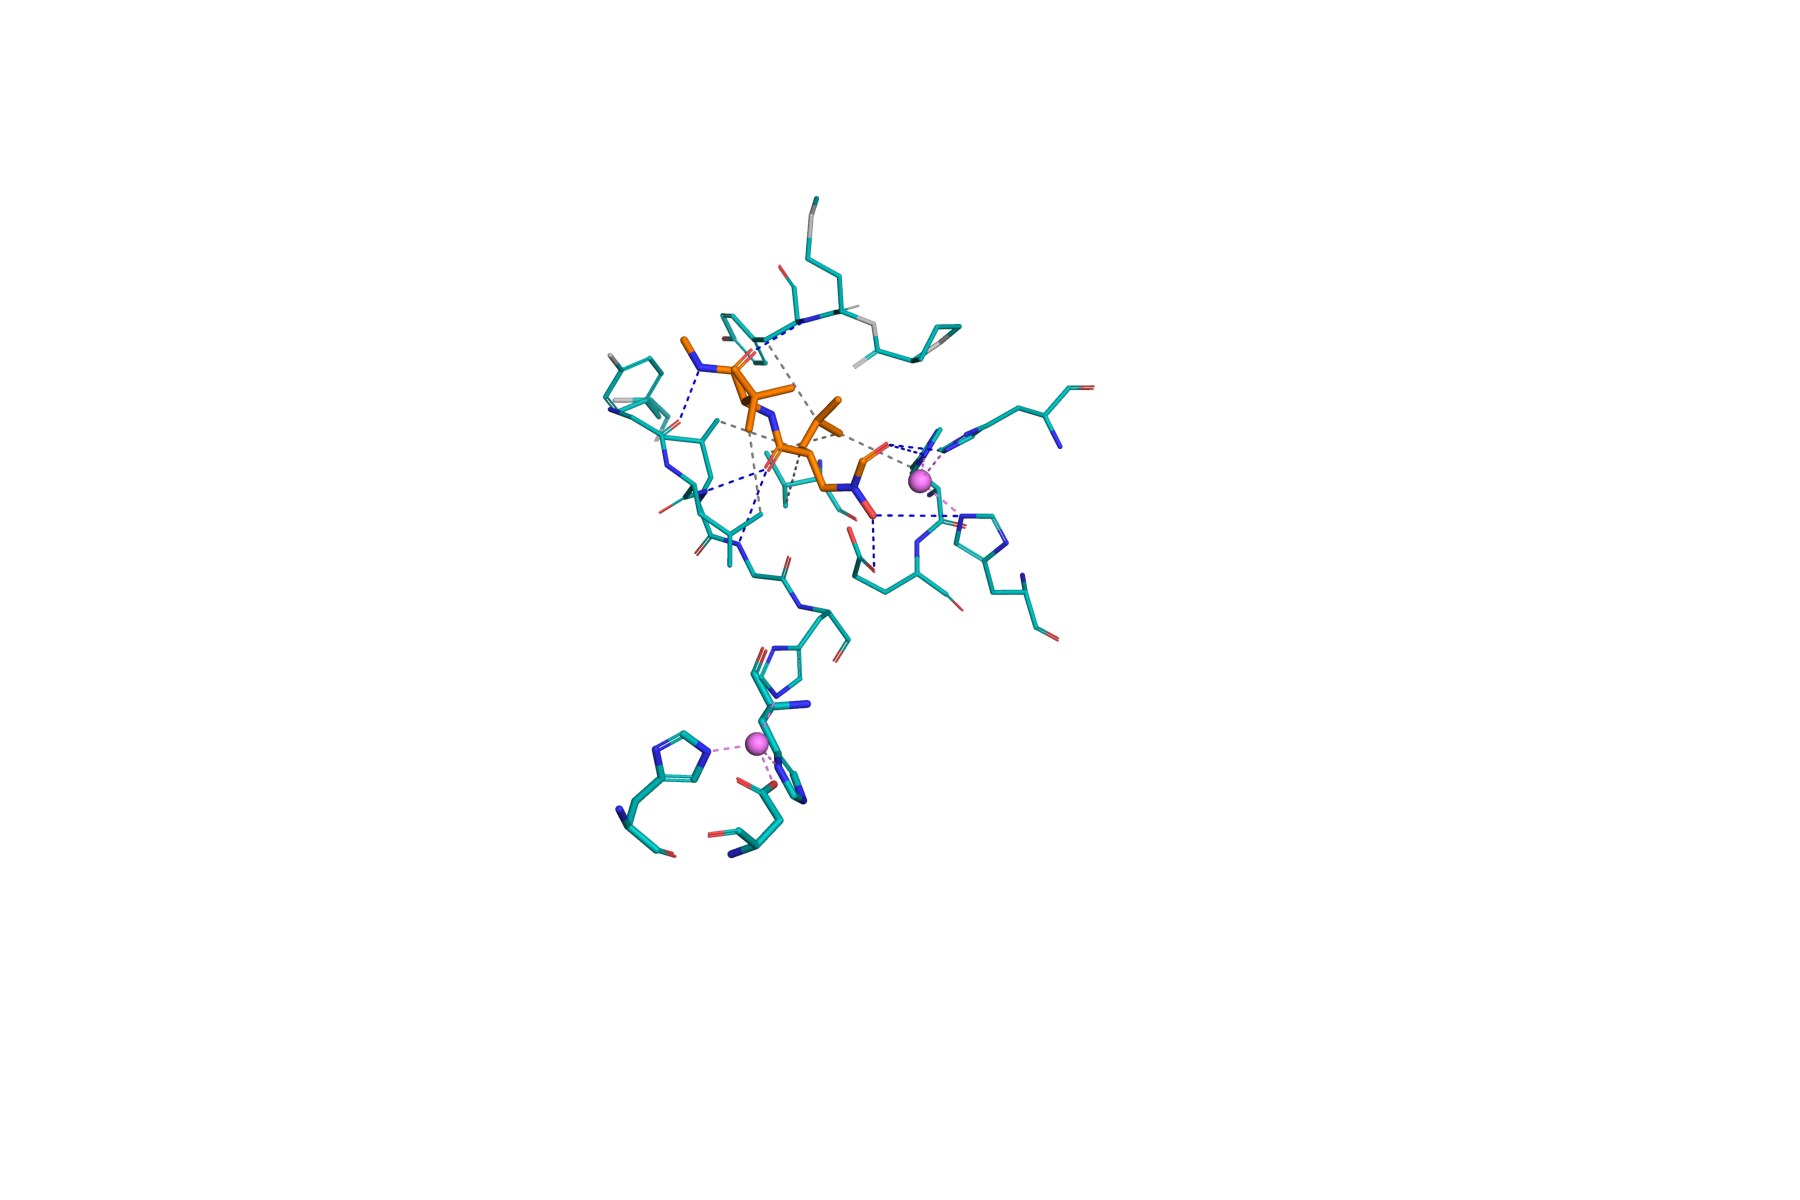
\includegraphics[width=0.64\linewidth,height=6cm,keepaspectratio,trim={138.72bp 75.84bp 163.20bp 41.04bp},clip]{image/redocking/1GKC_contatos_sem_tags.png}

\fonte{PyMOL 2.5.0.}
\end{figure}

\begin{figure}[H]\centering
\centering
\caption[Sobreposição de PLH em 1HFC]{Sobreposição de PLH com sua referência cristalográfica em 1HFC: pose 01, RMSD de 1,074~\AA.}\label{fig:fit_1HFC}
\par\centering\normalsize\begin{tabular}{@{}l@{\hspace{1.5em}}l@{}}\tikz[baseline=-.4ex]\filldraw[fill=orange,draw=black!40] (0,0) rectangle (.28,.28);\ Ligante dockado & \tikz[baseline=-.4ex]\filldraw[fill=forestgreen,draw=black!40] (0,0) rectangle (.28,.28);\ Ligante cristalográfico\end{tabular}\par\vspace{3pt}
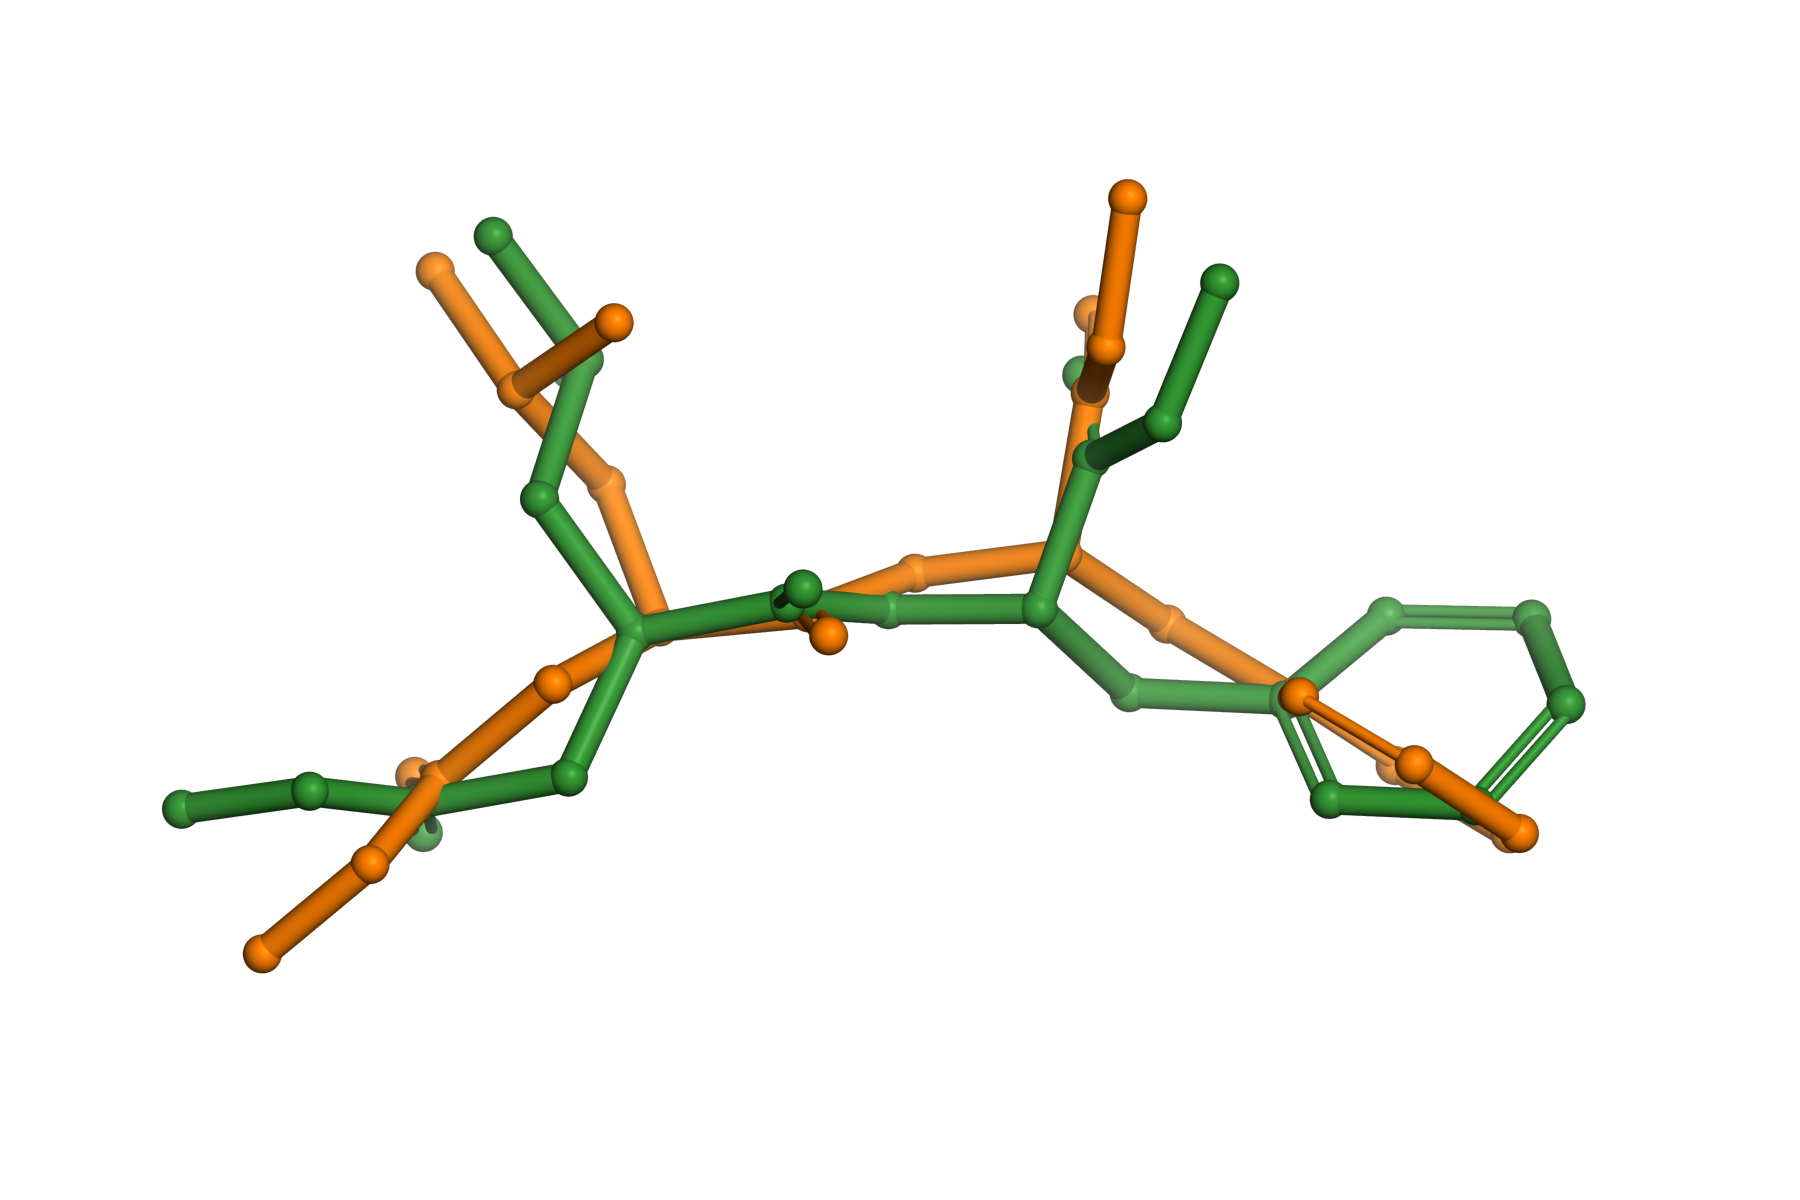
\includegraphics[width=.65\linewidth]{image/sobreposicoes_ligantes/1HFC_ligantes_sobrepostos.png}
\fonte{PyMOL 2.5.0.}
\vspace{6mm}
\centering
\caption[Contatos de PLH em 1HFC]{Contatos de PLH em 1HFC, pose 01.}\label{fig:redock_1HFC}

\par\centering\normalsize\begin{tabular}{@{}l@{\hspace{.5em}}l@{\hspace{1.5em}}l@{\hspace{.5em}}l@{}}
\definecolor{contatocor}{rgb}{0.5051,0.5051,0.5051}\tikz[baseline=-0.4ex]\draw[contatocor,line width=1.1pt,dashed] (0,0)--(0.7,0); & Contatos hidrofóbicos & \definecolor{contatocor}{rgb}{0.0,0.0,1.0}\tikz[baseline=-0.4ex]\draw[contatocor,line width=1.1pt,dashed] (0,0)--(0.7,0); & Ligações de hidrogênio\\[3pt]
\definecolor{contatocor}{rgb}{0.0,1.0,0.0}\tikz[baseline=-0.4ex]\draw[contatocor,line width=1.1pt,dashed] (0,0)--(0.7,0); & Empilhamento $\pi$ & \definecolor{contatocor}{rgb}{1.0,0.5,1.0}\tikz[baseline=-0.4ex]\draw[contatocor,line width=1.1pt,dashed] (0,0)--(0.7,0); & Coordenação de metais\\[3pt]
\tikz[baseline=-.4ex]{\filldraw[fill=orange,draw=black!40] (0,0) rectangle (.22,.22);} & Carbonos do ligante & \tikz[baseline=-.4ex]{\filldraw[fill=teal,draw=black!40] (0,0) rectangle (.22,.22);} & Carbonos dos resíduos\\[3pt]
\end{tabular}\par\vspace{3pt}
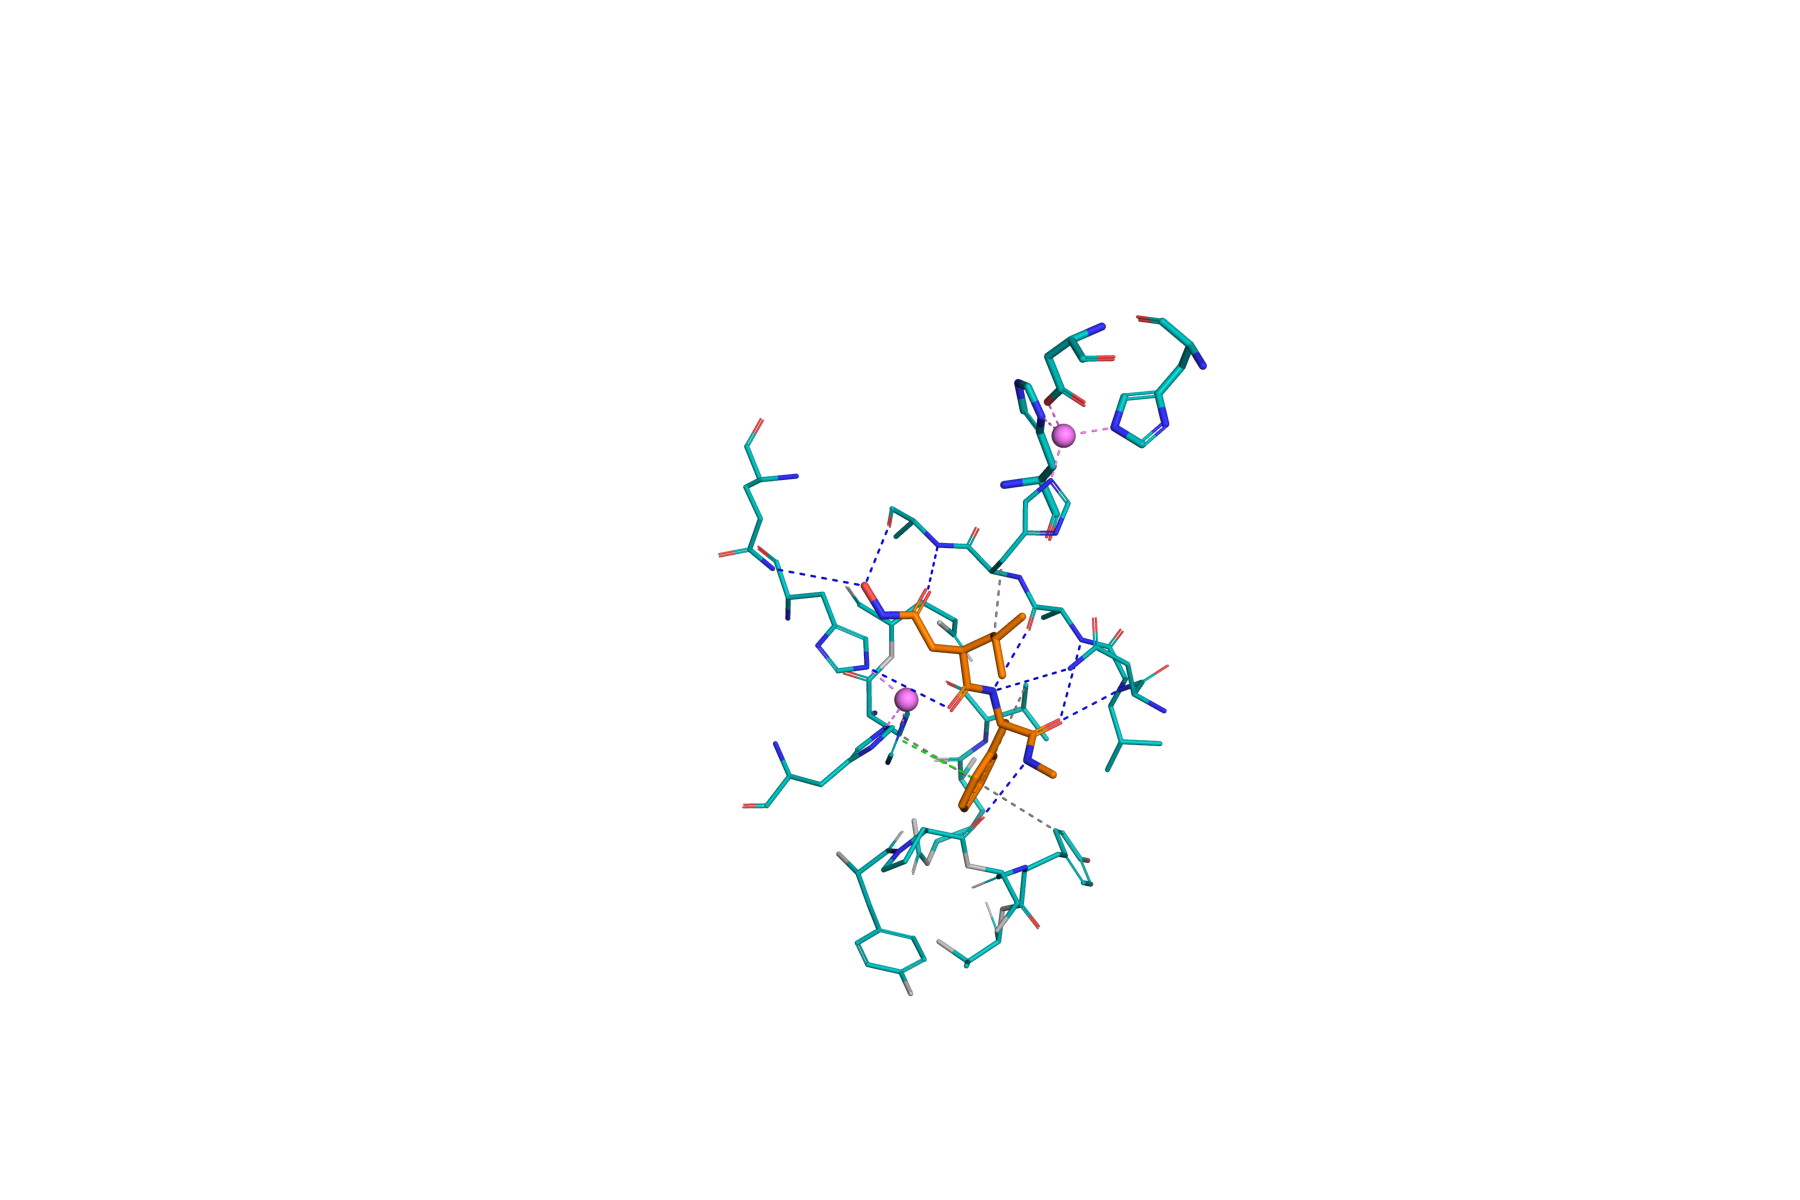
\includegraphics[width=0.64\linewidth,height=6cm,keepaspectratio,trim={166.32bp 42.72bp 136.32bp 69.60bp},clip]{image/redocking/1HFC_contatos_sem_tags.png}

\fonte{PyMOL 2.5.0.}
\end{figure}

\begin{figure}[H]\centering
\centering
\caption[L-tirosina em 5M8P: análise suplementar]{Sobreposição de L-tirosina em 5M8P: pose 03 de docking em laranja e referência cristalográfica em verde, com RMSD de 0,261~\AA. Análise suplementar, fora do conjunto de 34 ligantes.}\label{fig:fit_5M8P}
\par\centering\normalsize\begin{tabular}{@{}l@{\hspace{1.5em}}l@{}}\tikz[baseline=-.4ex]\filldraw[fill=orange,draw=black!40] (0,0) rectangle (.28,.28);\ Ligante dockado & \tikz[baseline=-.4ex]\filldraw[fill=forestgreen,draw=black!40] (0,0) rectangle (.28,.28);\ Ligante cristalográfico\end{tabular}\par\vspace{3pt}
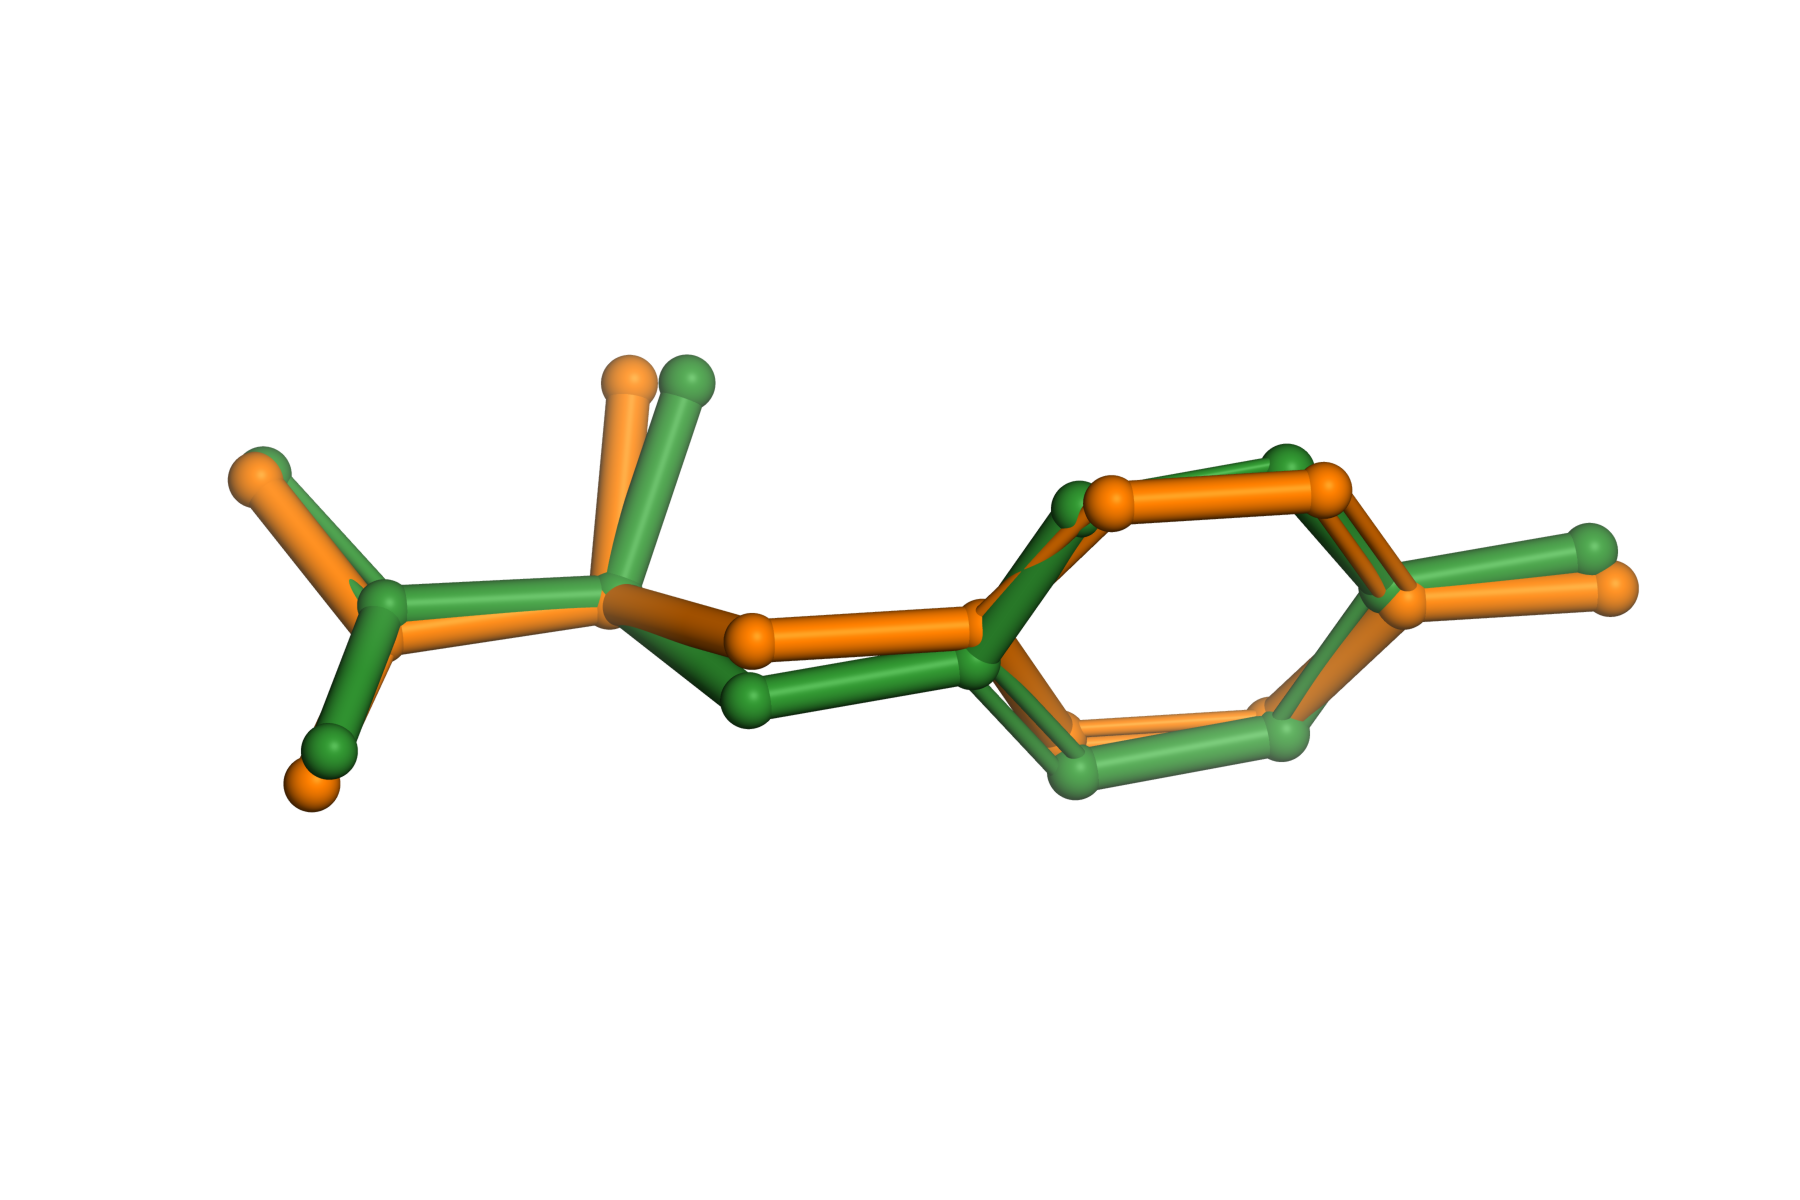
\includegraphics[width=.65\linewidth]{image/sobreposicoes_ligantes/5M8P_ligantes_sobrepostos.png}
\fonte{PyMOL 2.5.0.}
\vspace{6mm}
\centering
\caption[Contatos da L-tirosina em 5M8P]{Contatos da L-tirosina suplementar em 5M8P, pose 03; os carbonos do ligante estão em laranja.}\label{fig:redock_5M8P}

\par\centering\normalsize\begin{tabular}{@{}l@{\hspace{.5em}}l@{\hspace{1.5em}}l@{\hspace{.5em}}l@{}}
\definecolor{contatocor}{rgb}{0.5051,0.5051,0.5051}\tikz[baseline=-0.4ex]\draw[contatocor,line width=1.1pt,dashed] (0,0)--(0.7,0); & Contatos hidrofóbicos & \definecolor{contatocor}{rgb}{0.0,0.0,1.0}\tikz[baseline=-0.4ex]\draw[contatocor,line width=1.1pt,dashed] (0,0)--(0.7,0); & Ligações de hidrogênio\\[3pt]
\definecolor{contatocor}{rgb}{1.0,0.5,1.0}\tikz[baseline=-0.4ex]\draw[contatocor,line width=1.1pt,dashed] (0,0)--(0.7,0); & Coordenação de metais & \tikz[baseline=-.4ex]{\filldraw[fill=orange,draw=black!40] (0,0) rectangle (.22,.22);} & Carbonos do ligante\\[3pt]
\multicolumn{4}{c}{\tikz[baseline=-.4ex]{\filldraw[fill=teal,draw=black!40] (0,0) rectangle (.22,.22);}\hspace{.5em}Carbonos dos resíduos}\\[3pt]
\end{tabular}\par\vspace{3pt}
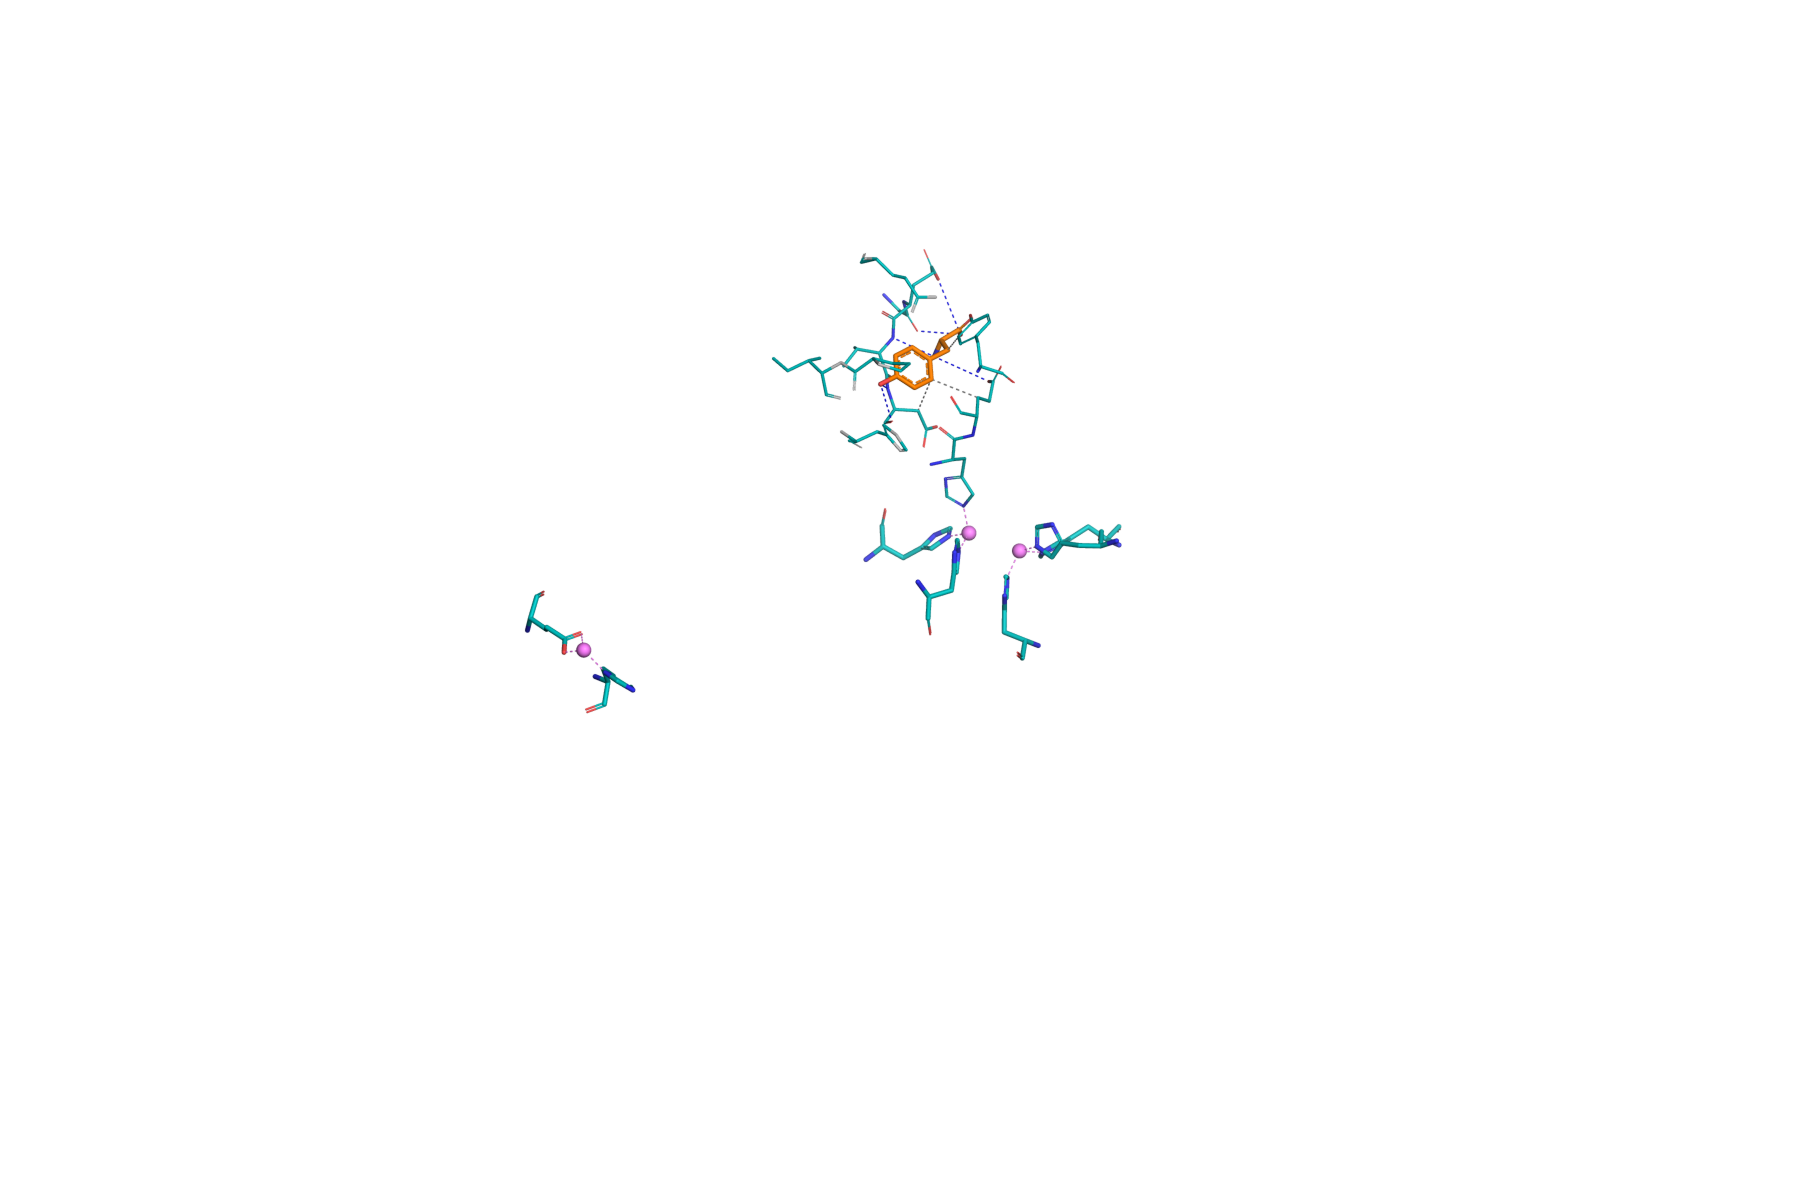
\includegraphics[width=0.64\linewidth,height=6cm,keepaspectratio,trim={120.00bp 110.64bp 156.72bp 53.76bp},clip]{image/redocking/5M8P_contatos_sem_tags.png}

\fonte{PyMOL 2.5.0.}
\end{figure}

\begin{figure}[H]\centering
\centering
\caption[Sobreposição de L2U em 8H78]{Sobreposição de L2U com sua referência cristalográfica em 8H78: pose 04, RMSD de 3,451~\AA.}\label{fig:fit_8H78}
\par\centering\normalsize\begin{tabular}{@{}l@{\hspace{1.5em}}l@{}}\tikz[baseline=-.4ex]\filldraw[fill=orange,draw=black!40] (0,0) rectangle (.28,.28);\ Ligante dockado & \tikz[baseline=-.4ex]\filldraw[fill=forestgreen,draw=black!40] (0,0) rectangle (.28,.28);\ Ligante cristalográfico\end{tabular}\par\vspace{3pt}
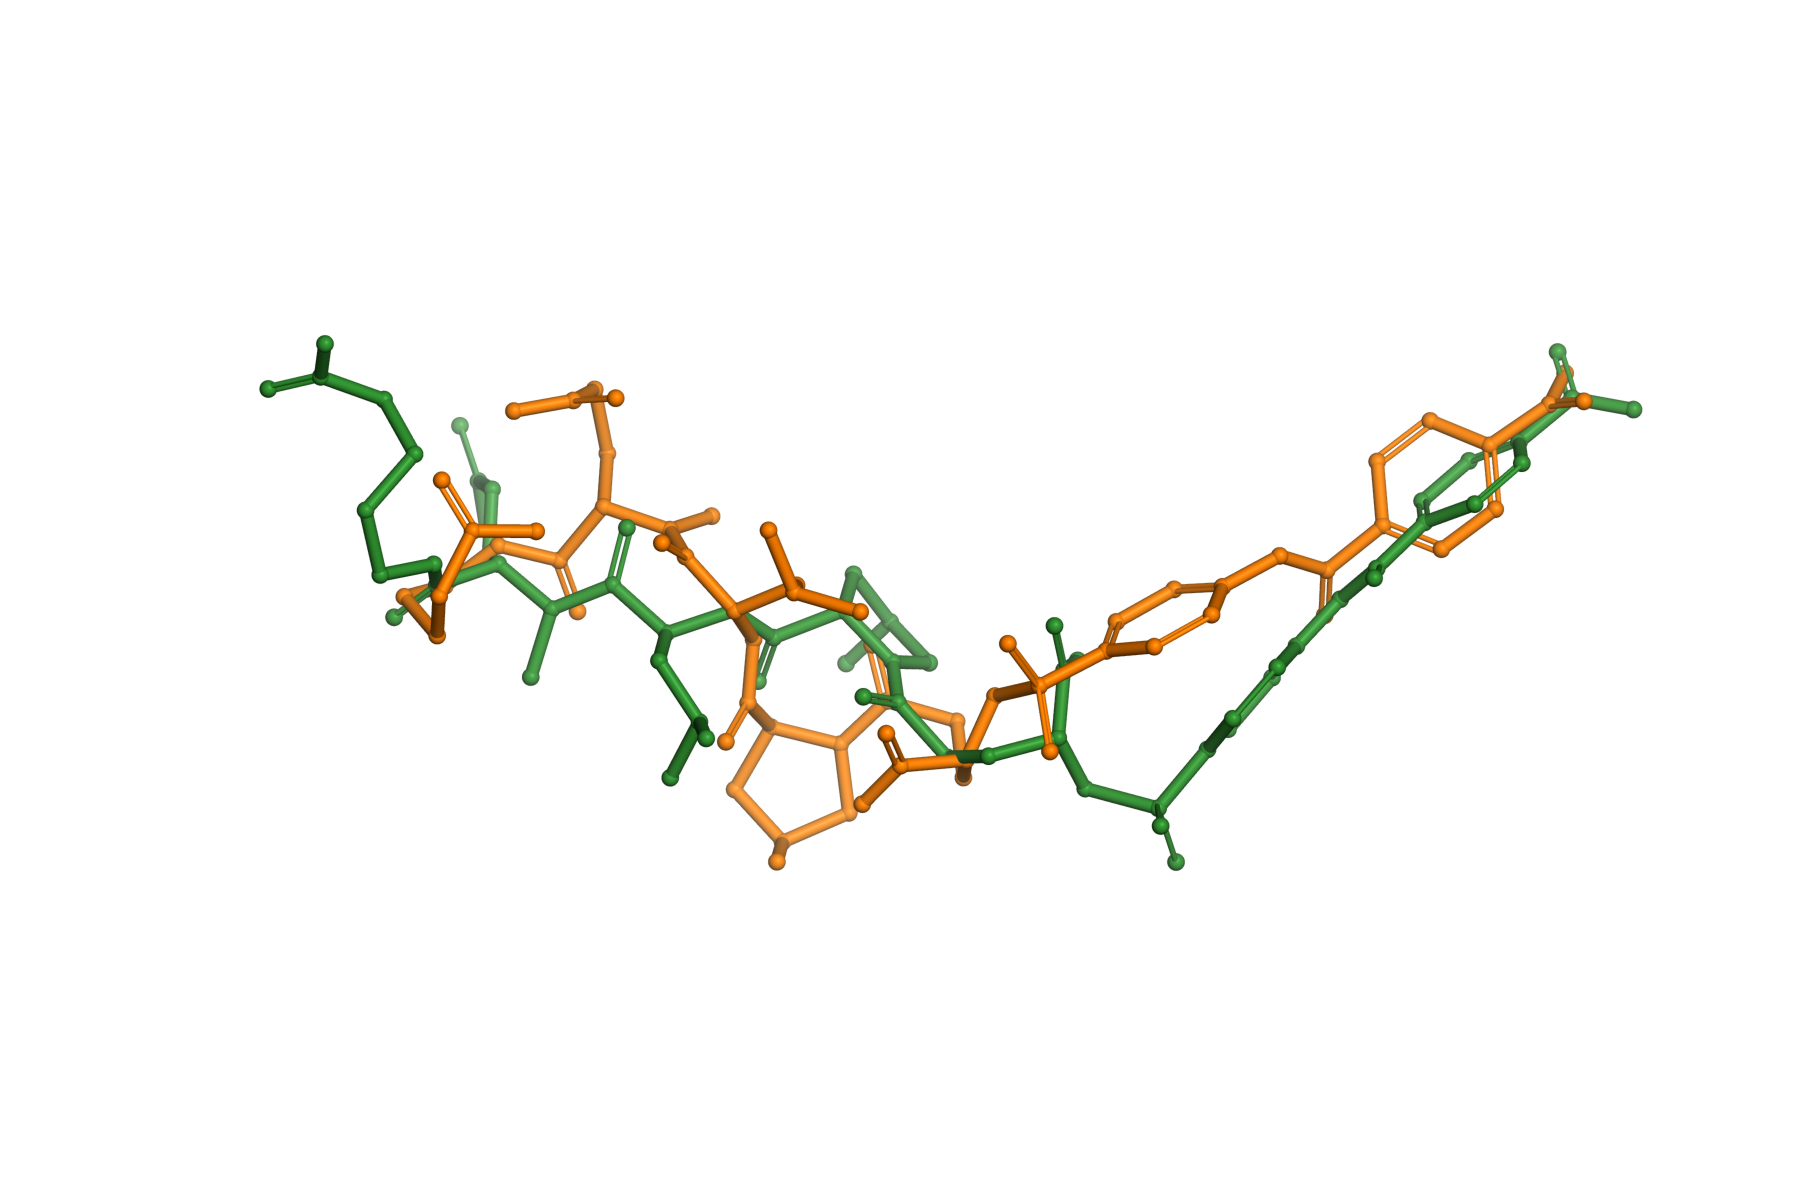
\includegraphics[width=.65\linewidth]{image/sobreposicoes_ligantes/8H78_ligantes_sobrepostos.png}
\fonte{PyMOL 2.5.0.}
\vspace{6mm}
\centering
\caption[Contatos de L2U em 8H78]{Contatos de L2U em 8H78, pose 04.}\label{fig:redock_8H78}

\par\centering\normalsize\begin{tabular}{@{}l@{\hspace{.5em}}l@{\hspace{1.5em}}l@{\hspace{.5em}}l@{}}
\definecolor{contatocor}{rgb}{0.5051,0.5051,0.5051}\tikz[baseline=-0.4ex]\draw[contatocor,line width=1.1pt,dashed] (0,0)--(0.7,0); & Contatos hidrofóbicos & \definecolor{contatocor}{rgb}{0.0,0.0,1.0}\tikz[baseline=-0.4ex]\draw[contatocor,line width=1.1pt,dashed] (0,0)--(0.7,0); & Ligações de hidrogênio\\[3pt]
\definecolor{contatocor}{rgb}{1.0,0.87,0.37}\tikz[baseline=-0.4ex]\draw[contatocor,line width=1.1pt,dashed] (0,0)--(0.7,0); & Pontes salinas & \definecolor{contatocor}{rgb}{0.0,1.0,0.0}\tikz[baseline=-0.4ex]\draw[contatocor,line width=1.1pt,dashed] (0,0)--(0.7,0); & Empilhamento $\pi$\\[3pt]
\definecolor{contatocor}{rgb}{1.0,0.5,1.0}\tikz[baseline=-0.4ex]\draw[contatocor,line width=1.1pt,dashed] (0,0)--(0.7,0); & Coordenação de metais & \tikz[baseline=-.4ex]{\filldraw[fill=orange,draw=black!40] (0,0) rectangle (.22,.22);} & Carbonos do ligante\\[3pt]
\multicolumn{4}{c}{\tikz[baseline=-.4ex]{\filldraw[fill=teal,draw=black!40] (0,0) rectangle (.22,.22);}\hspace{.5em}Carbonos dos resíduos}\\[3pt]
\end{tabular}\par\vspace{3pt}
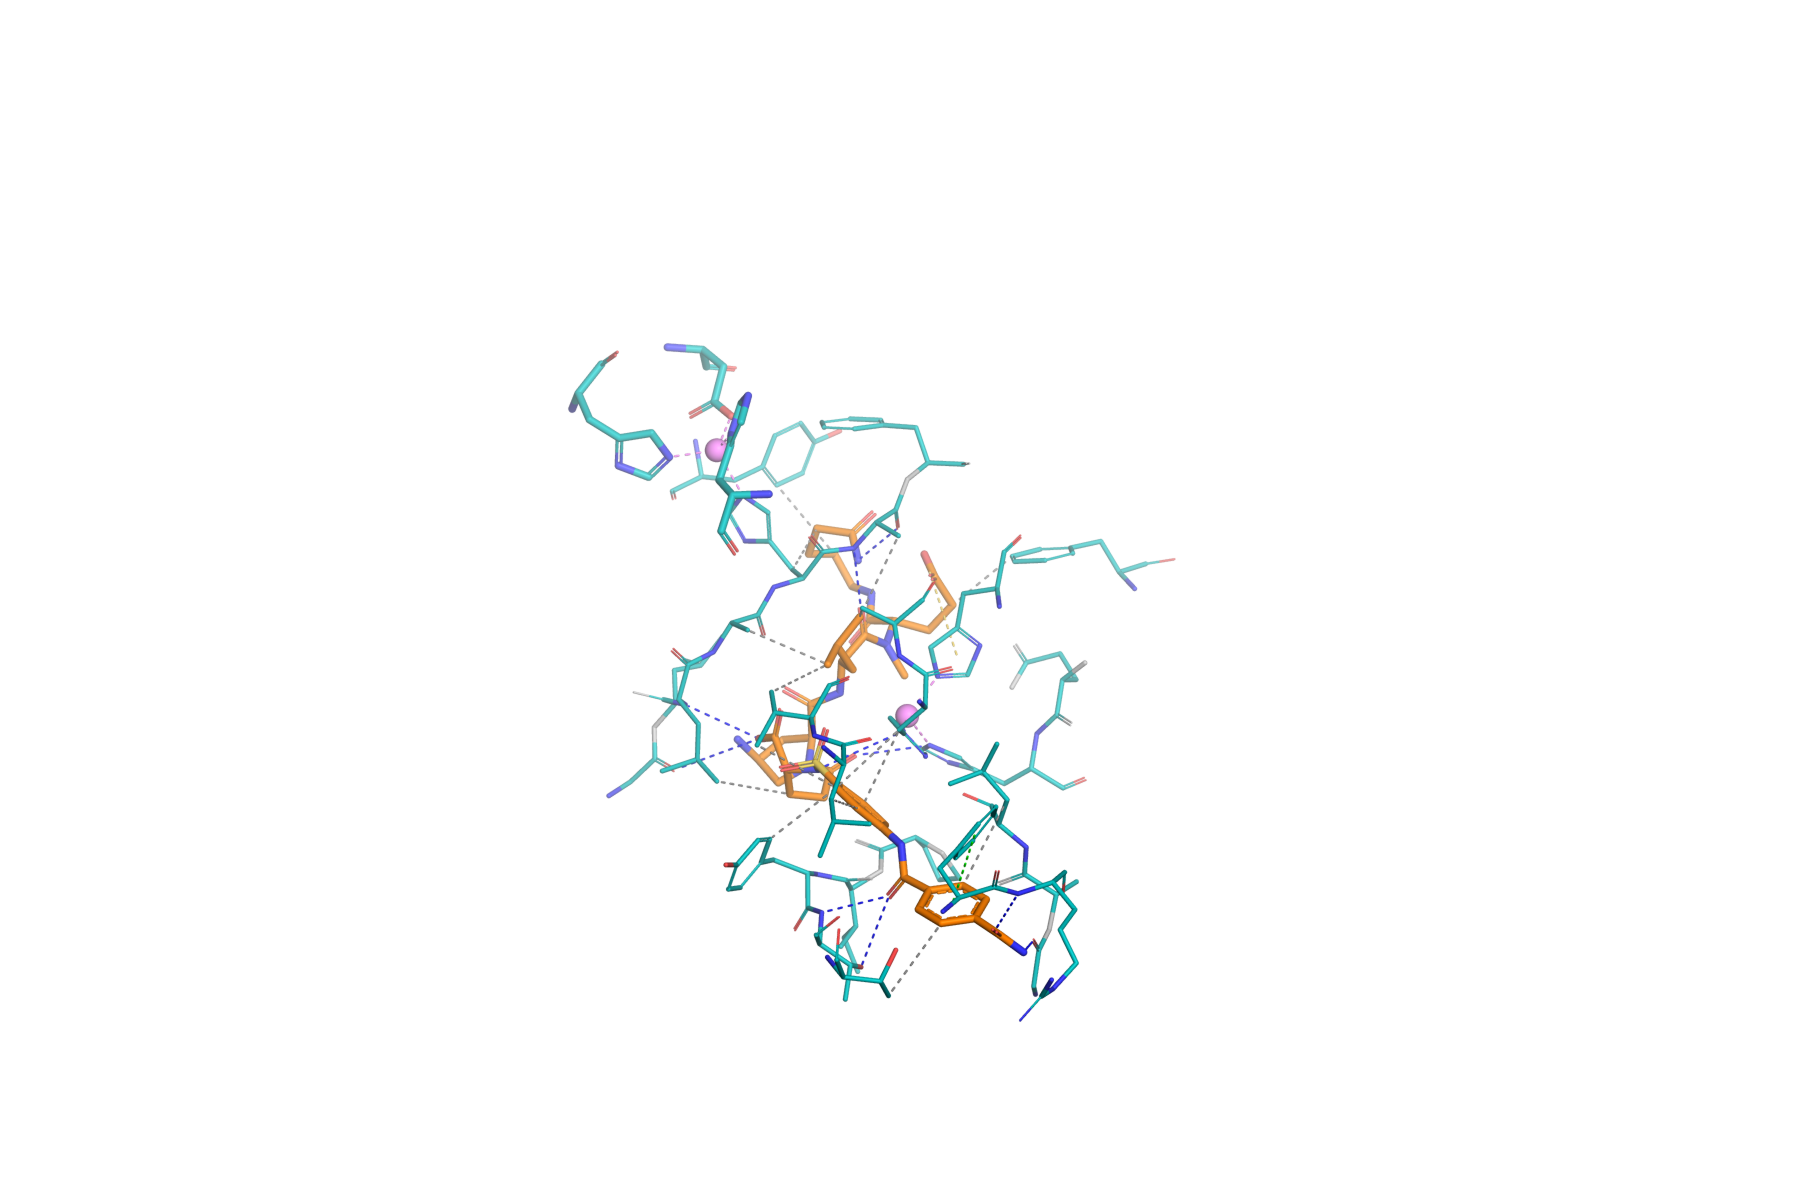
\includegraphics[width=0.64\linewidth,height=6cm,keepaspectratio,trim={130.32bp 36.72bp 143.76bp 76.32bp},clip]{image/redocking/8H78_contatos_sem_tags.png}

\fonte{PyMOL 2.5.0.}
\end{figure}

\begin{figure}[H]\centering
\centering
\caption[Sobreposição de GW475151 em 1H1B]{Sobreposição de GW475151 com sua referência cristalográfica em 1H1B na execução anterior: pose 03, RMSD de 1,836~\AA.}\label{fig:fit_1H1B}
\par\centering\normalsize\begin{tabular}{@{}l@{\hspace{1.5em}}l@{}}\tikz[baseline=-.4ex]\filldraw[fill=orange,draw=black!40] (0,0) rectangle (.28,.28);\ Ligante dockado & \tikz[baseline=-.4ex]\filldraw[fill=forestgreen,draw=black!40] (0,0) rectangle (.28,.28);\ Ligante cristalográfico\end{tabular}\par\vspace{3pt}
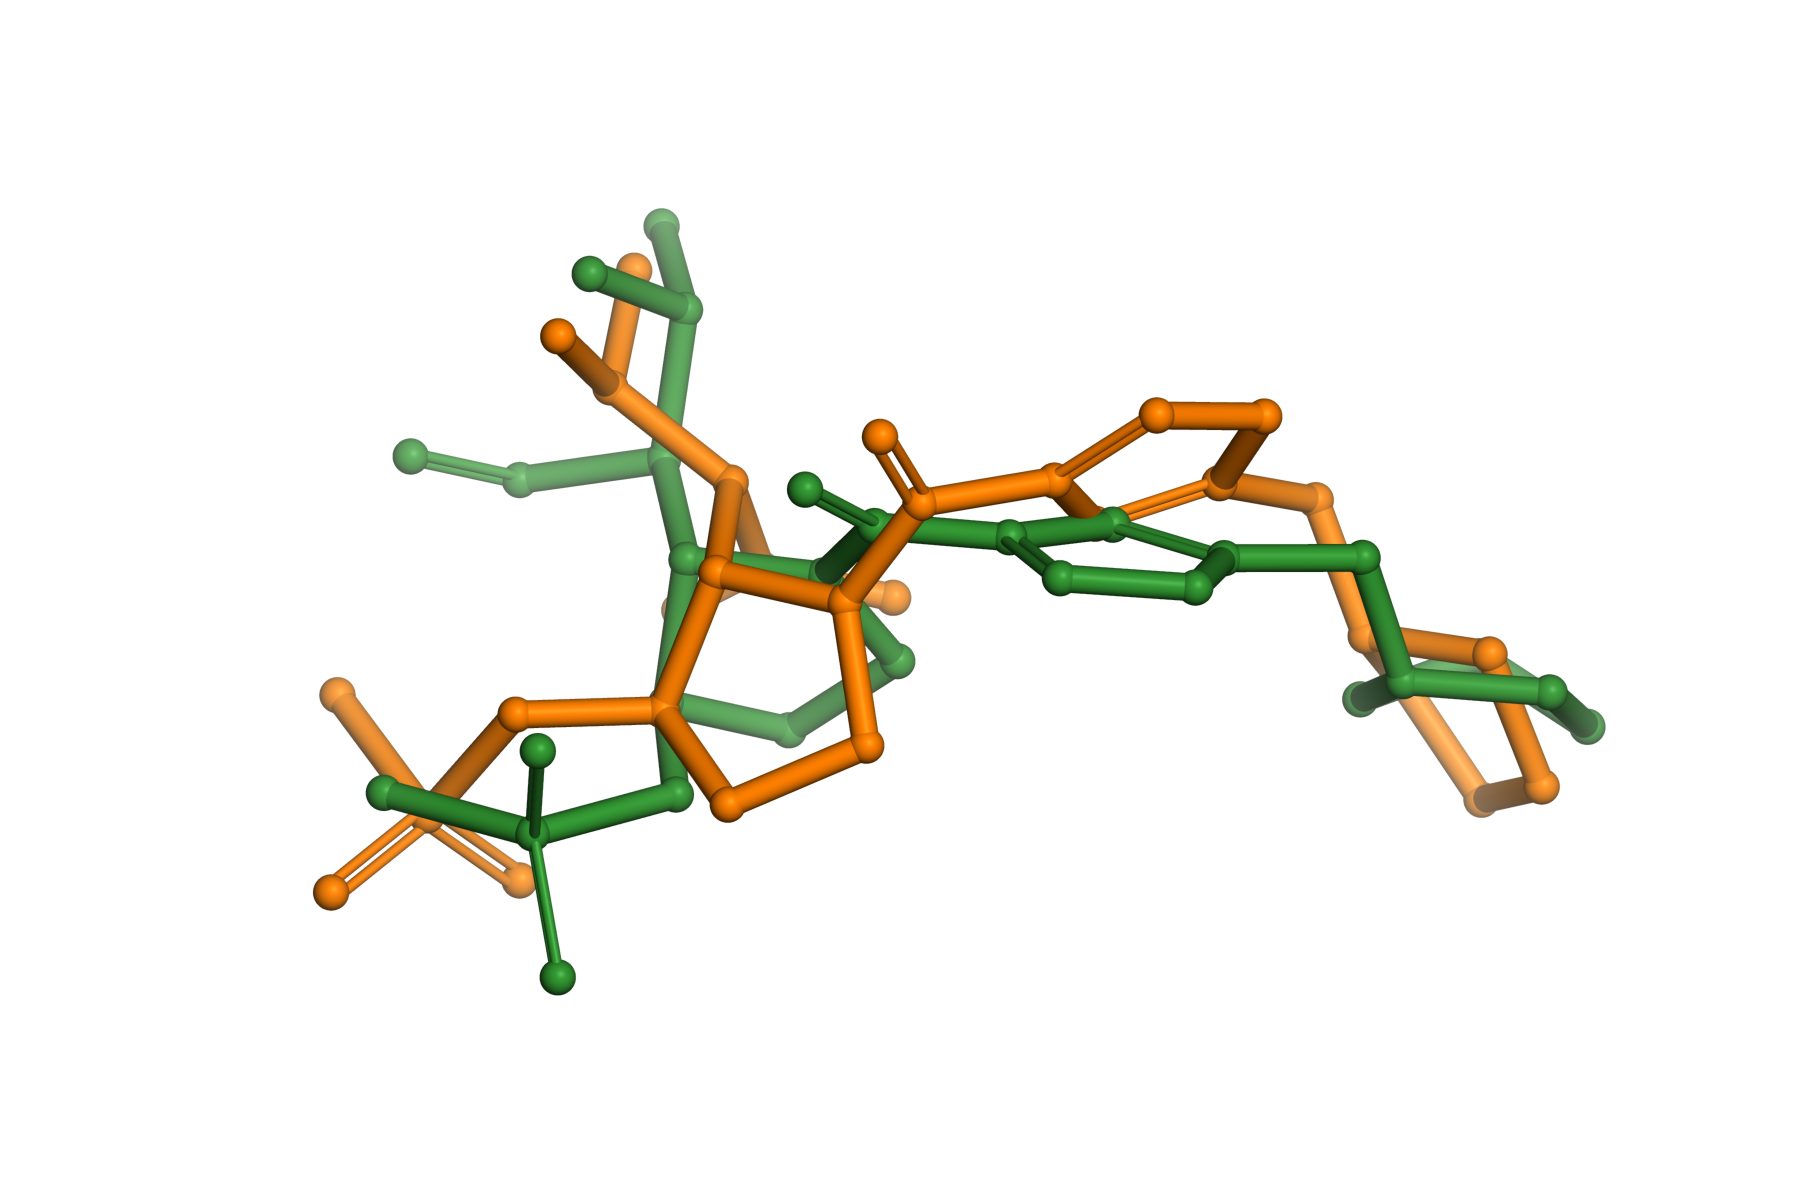
\includegraphics[width=.65\linewidth]{image/sobreposicoes_ligantes/1H1B_ligantes_sobrepostos.png}
\fonte{PyMOL 2.5.0.}
\vspace{6mm}
\centering
\caption[Contatos de GW475151 em 1H1B]{Contatos de GW475151 em 1H1B, pose 03 da execução anterior.}\label{fig:redock_1H1B}

\par\centering\normalsize\begin{tabular}{@{}l@{\hspace{.5em}}l@{\hspace{1.5em}}l@{\hspace{.5em}}l@{}}
\definecolor{contatocor}{rgb}{0.5051,0.5051,0.5051}\tikz[baseline=-0.4ex]\draw[contatocor,line width=1.1pt,dashed] (0,0)--(0.7,0); & Contatos hidrofóbicos & \definecolor{contatocor}{rgb}{0.0,0.0,1.0}\tikz[baseline=-0.4ex]\draw[contatocor,line width=1.1pt,dashed] (0,0)--(0.7,0); & Ligações de hidrogênio\\[3pt]
\definecolor{contatocor}{rgb}{1.0,0.5,0.0}\tikz[baseline=-0.4ex]\draw[contatocor,line width=1.1pt,dashed] (0,0)--(0.7,0); & Interações $\pi$--cátion & \tikz[baseline=-.4ex]{\filldraw[fill=orange,draw=black!40] (0,0) rectangle (.22,.22);} & Carbonos do ligante\\[3pt]
\multicolumn{4}{c}{\tikz[baseline=-.4ex]{\filldraw[fill=teal,draw=black!40] (0,0) rectangle (.22,.22);}\hspace{.5em}Carbonos dos resíduos}\\[3pt]
\end{tabular}\par\vspace{3pt}
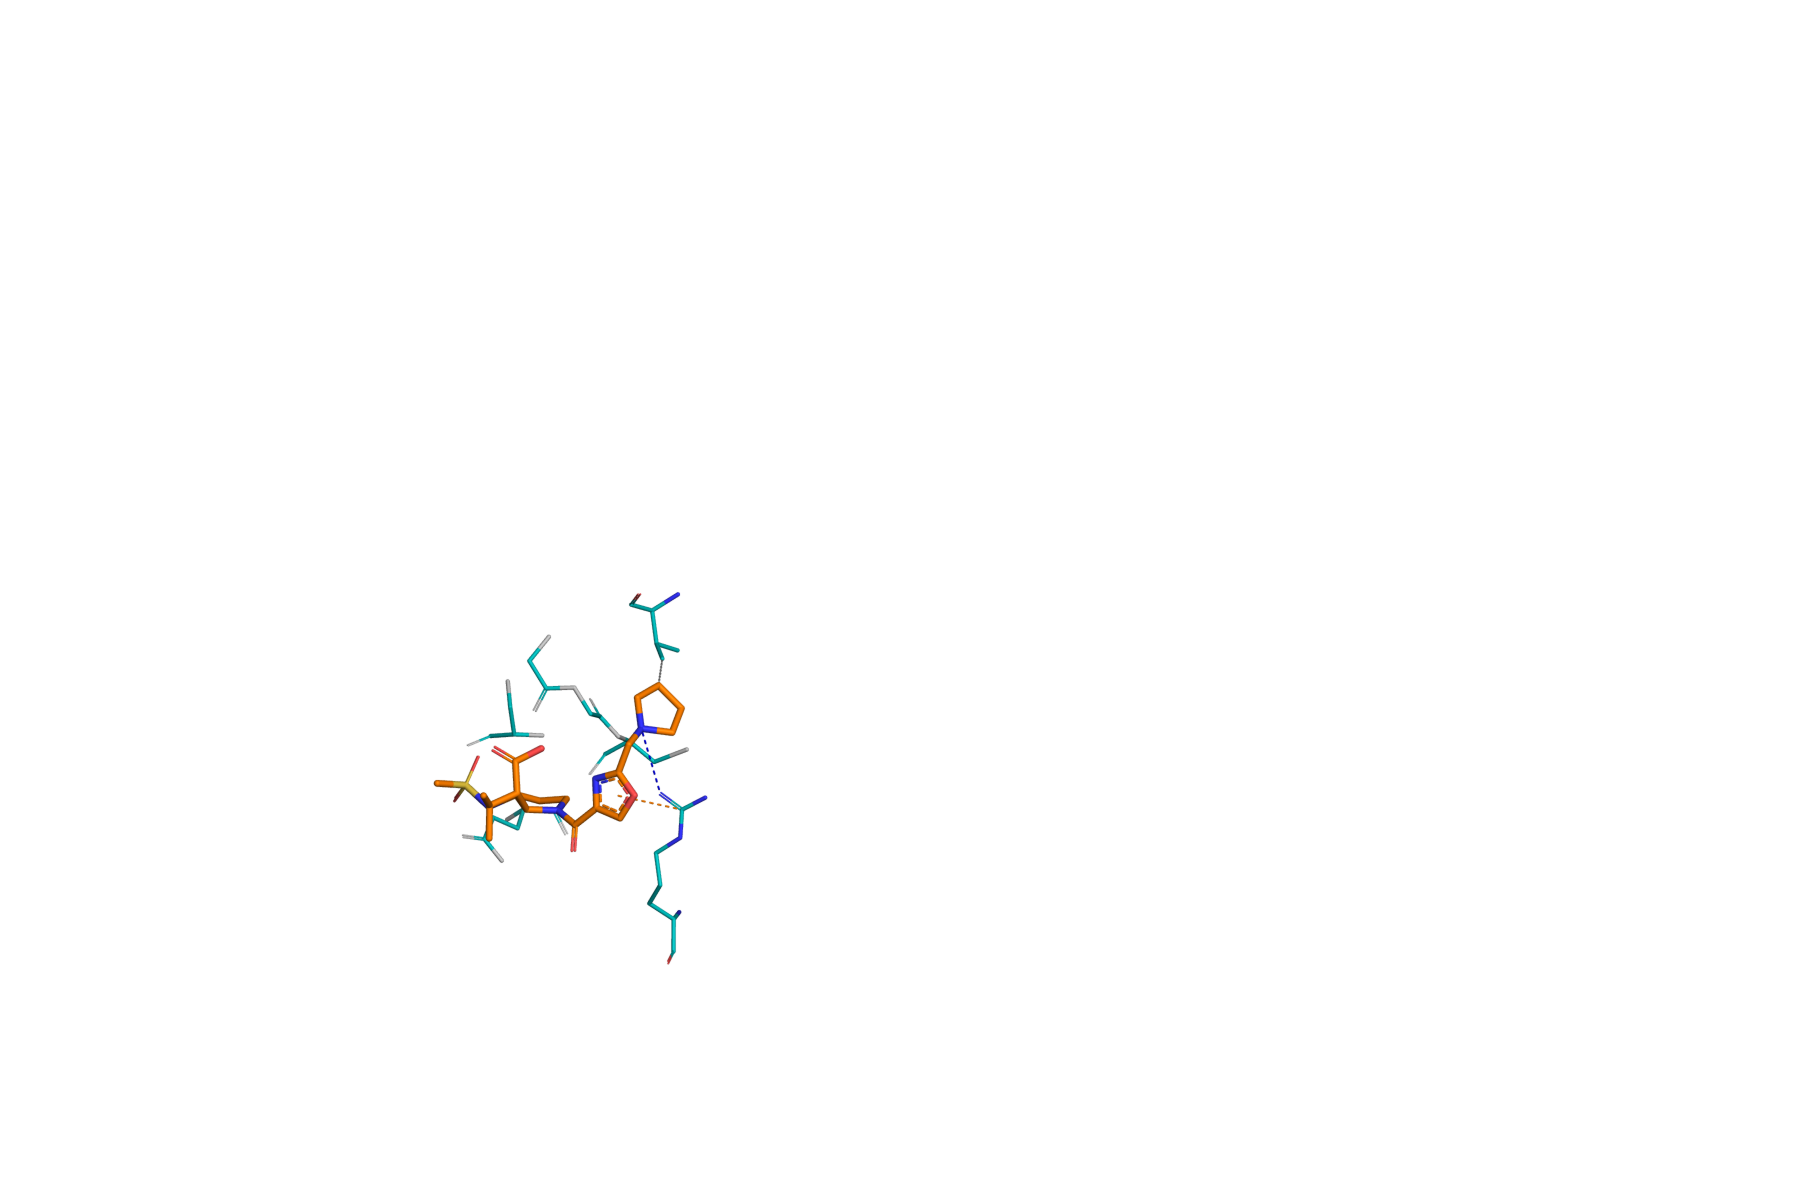
\includegraphics[width=0.64\linewidth,height=6cm,keepaspectratio,trim={97.92bp 50.40bp 256.08bp 136.08bp},clip]{image/redocking/1H1B_contatos_sem_tags.png}

\fonte{PyMOL 2.5.0.}
\end{figure}

\subsection{Resultados por receptor e perfil de interações}
Os resultados são organizados por receptor. Primeiro são discutidas as metaloproteinases MMP-9 (1GKC), MMP-1 (1HFC) e MMP-2 (8H78), seguidas de TYRP1 (5M8P); elastase (1H1B) e hialuronidase 1 (2PE4) encerram a sequência. As Figuras~\ref{fig:lollipop_1GKC}, \ref{fig:lollipop_1HFC}, \ref{fig:lollipop_8H78}, \ref{fig:lollipop_5M8P}, \ref{fig:lollipop_1H1B} e~\ref{fig:lollipop_2PE4} apresentam os 34 ligantes de cada receptor em ordem crescente de FEB, da pontuação mais negativa à menos negativa. O azul identifica os ligantes comerciais e coocristalizados; o vinho, os compostos selecionados para prospecção. Nas matrizes, cada marca indica a presença de um contato entre ligante e resíduo, e as colunas seguem a recorrência decrescente dos resíduos. A FEB ordena as poses segundo a função de pontuação, enquanto as matrizes descrevem a distribuição dos contatos previstos; ambas são comparadas dentro de cada receptor \parencite{salentin2015plip,warren2006}.

\FloatBarrier
\subsubsection{Gelatinase B humana (MMP-9, 1GKC)}
A comparação conformacional de NFH com o ligante cristalográfico fornece uma referência estrutural para a análise de MMP-9. No conjunto de prospecção, o destaque da glicose-6-sulfato motivou o exame de sua pose e dos contatos de seus grupos polares com o receptor. Essa análise descreve a acomodação da molécula isolada no modelo, sem atribuir seu resultado aos polissacarídeos de \textit{T. chuii} \parencite{rowsell2002,warren2006}.
Nos relatórios PLIP das poses selecionadas, PRO~421 da cadeia A aparece em cinco registros para L2U e em três para glicose-6-sulfato. Na matriz, cada par ligante--resíduo conta uma única vez; portanto, os dois ligantes apresentam contato com PRO~421, e os números de registros descrevem o detalhamento dos relatórios.



\begin{figure}[H]
\centering
\caption[Docking em MMP-9 (1GKC)]{Pontuações de docking (FEB, kcal/mol) dos 34 ligantes para a gelatinase B humana (MMP-9, 1GKC).}\label{fig:lollipop_1GKC}
\par\vspace{2pt}\begin{tabular}{@{}l@{\hspace{1.5em}}l@{}}\tikz[baseline=-.4ex]\filldraw[fill=mapacomercial,draw=black!40] (0,0) rectangle (.28,.28);\ Ligantes comerciais e coocristalizados & \tikz[baseline=-.4ex]\filldraw[fill=mapatetra,draw=black!40] (0,0) rectangle (.28,.28);\ Prospecção\end{tabular}\par\vspace{2pt}
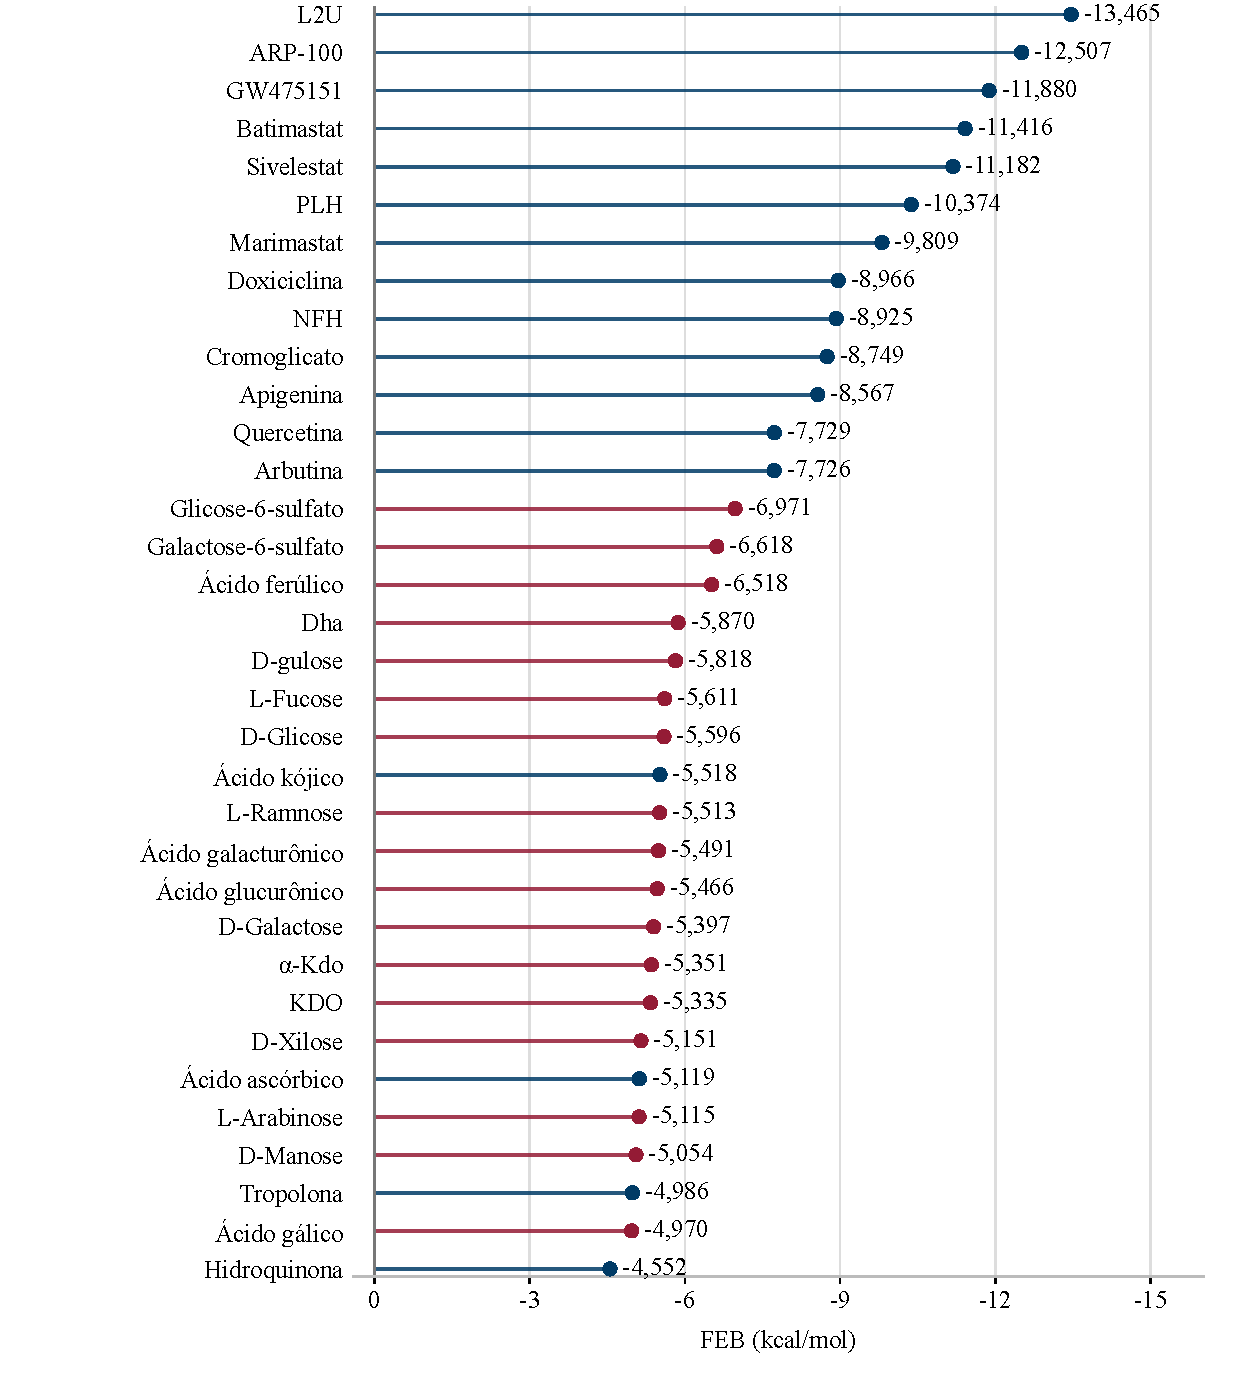
\includegraphics[width=\linewidth,height=17.5cm,keepaspectratio]{image/lollipop/lollipop_1GKC.pdf}
\end{figure}

Na Figura~\ref{fig:lollipop_1GKC}, L2U (-13,465~kcal/mol) e ARP-100 (-12,507~kcal/mol) ocupam as primeiras posições do conjunto de ligantes comerciais e coocristalizados. No conjunto de prospecção, as menores FEB foram obtidas para glicose-6-sulfato (-6,971~kcal/mol), galactose-6-sulfato (-6,618~kcal/mol) e ácido ferúlico (-6,518~kcal/mol). A glicose-6-sulfato ficou na 14ª posição geral, com pontuação 6,494~kcal/mol menos negativa que a de L2U. Assim, ela lidera o conjunto de prospecção, enquanto L2U ocupa a primeira posição na classificação conjunta.

As medianas de FEB foram -8,925~kcal/mol para o conjunto de ligantes comerciais e coocristalizados e -5,491~kcal/mol para o conjunto de prospecção. A mediana mais negativa dos ligantes comerciais e coocristalizados mostra que a diferença entre os conjuntos também aparece no centro das distribuições. A sobreposição das faixas de pontuação mostra, contudo, que alguns compostos do conjunto de prospecção se posicionaram à frente de parte dos ligantes comerciais e coocristalizados. Essa sobreposição permite priorizar compostos do conjunto de prospecção para examinar suas poses e seus contatos em relação aos ligantes comerciais e coocristalizados.


Na Figura~\ref{fig:mapa_interacoes_1GKC}, ALA~189, LEU~188 e GLU~402 da cadeia A apresentam contatos com 24, 21 e 20 ligantes, respectivamente. A concentração de presenças nessas colunas indica resíduos compartilhados por diferentes poses, enquanto as demais colunas mostram contatos menos recorrentes. Essas frequências descrevem a distribuição dos contatos, sem estabelecer a contribuição energética de cada resíduo.

A distribuição por grupo destacou ALA~189, com contato em 12 ligantes comerciais e coocristalizados e 12 compostos em prospecção, e LEU~188, com contato em 12 e 9 ligantes, respectivamente; ambos pertencem à cadeia A. A recorrência idêntica de ALA~189 evidencia um contato comum aos dois conjuntos. GLU~402 foi mais recorrente no conjunto de prospecção, cuja mediana de FEB foi menos negativa. Esse contraste mostra que a frequência de um resíduo, isoladamente, não explica a classificação por FEB.

\begin{figure}[H]\centering
\caption[Matriz de contatos em MMP-9 (1GKC)]{Matriz de presença das interações dos 34 ligantes com os resíduos de MMP-9 (1GKC).}\label{fig:mapa_interacoes_1GKC}
\par\vspace{3pt}\begin{tabular}{@{}l@{\hspace{1em}}l@{\hspace{1em}}l@{}}\tikz[baseline=-.4ex]\filldraw[fill=mapacomercial,draw=black!40] (0,0) rectangle (.28,.28);\ Comerciais e coocristalizados & \tikz[baseline=-.4ex]\filldraw[fill=mapatetra,draw=black!40] (0,0) rectangle (.28,.28);\ Prospecção & \tikz[baseline=-.4ex]\filldraw[fill=white,draw=black!40] (0,0) rectangle (.28,.28);\ Sem contato registrado\end{tabular}\par\vspace{3pt}\normalsize X: contato presente.\par\vspace{5pt}
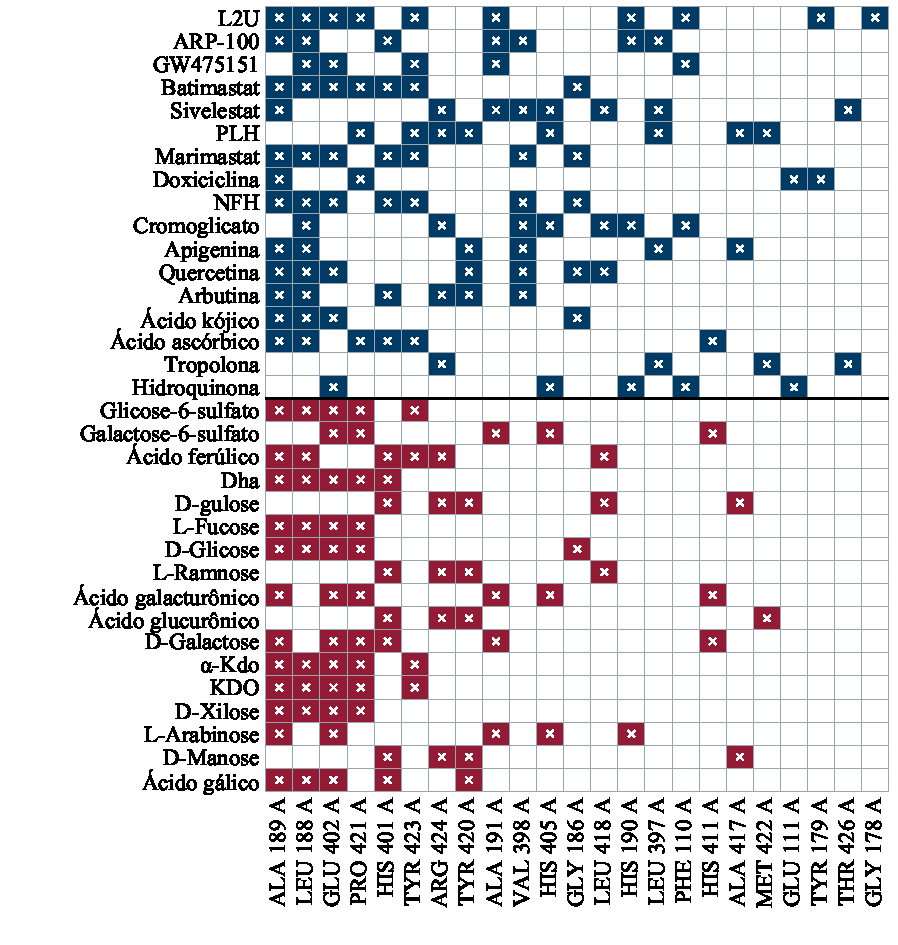
\includegraphics[width=15.2cm,height=14cm,keepaspectratio]{image/interacoes/mapa_interacoes_1GKC.pdf}
\fonte{Relatórios PLIP da matriz principal. Resíduos da cadeia A, ordenados pelo número decrescente de ligantes com interação; empates por número do resíduo.}
\end{figure}

Na comparação direta, L2U contatou dez resíduos e a glicose-6-sulfato, cinco. Os cinco resíduos da pose do açúcar também aparecem na pose de L2U: PRO~421, TYR~423, LEU~188, ALA~189 e GLU~402. L2U apresentou ainda contatos com PHE~110, TYR~179, HIS~190, GLY~178 e ALA~191. A FEB da glicose-6-sulfato foi 6,494~kcal/mol menos negativa que a de L2U.





\FloatBarrier
\subsubsection{Colagenase de fibroblastos humanos (MMP-1, 1HFC)}
A glicose-6-sulfato apresentou FEB de -7,591~kcal/mol e liderou o conjunto de prospecção em MMP-1. Seu destaque também em MMP-9 é um padrão da classificação, mas não permite inferir seletividade entre as duas proteínas. A sobreposição de PLH apresentada anteriormente descreve semelhança conformacional e não a recuperação da orientação cristalográfica no sítio \parencite{spurlino1994,cole2005,warren2006}.
O relatório PLIP da pose selecionada lista dois registros de contato entre GLU~219 da cadeia A e glicose-6-sulfato. Na matriz, esse par é contado uma única vez; o número de registros descreve o detalhamento do relatório, não a contribuição energética do resíduo.



\begin{figure}[H]
\centering
\caption[Docking em MMP-1 (1HFC)]{Pontuações de docking (FEB, kcal/mol) dos 34 ligantes para a colagenase humana (MMP-1, 1HFC).}\label{fig:lollipop_1HFC}
\par\vspace{2pt}\begin{tabular}{@{}l@{\hspace{1.5em}}l@{}}\tikz[baseline=-.4ex]\filldraw[fill=mapacomercial,draw=black!40] (0,0) rectangle (.28,.28);\ Ligantes comerciais e coocristalizados & \tikz[baseline=-.4ex]\filldraw[fill=mapatetra,draw=black!40] (0,0) rectangle (.28,.28);\ Prospecção\end{tabular}\par\vspace{2pt}
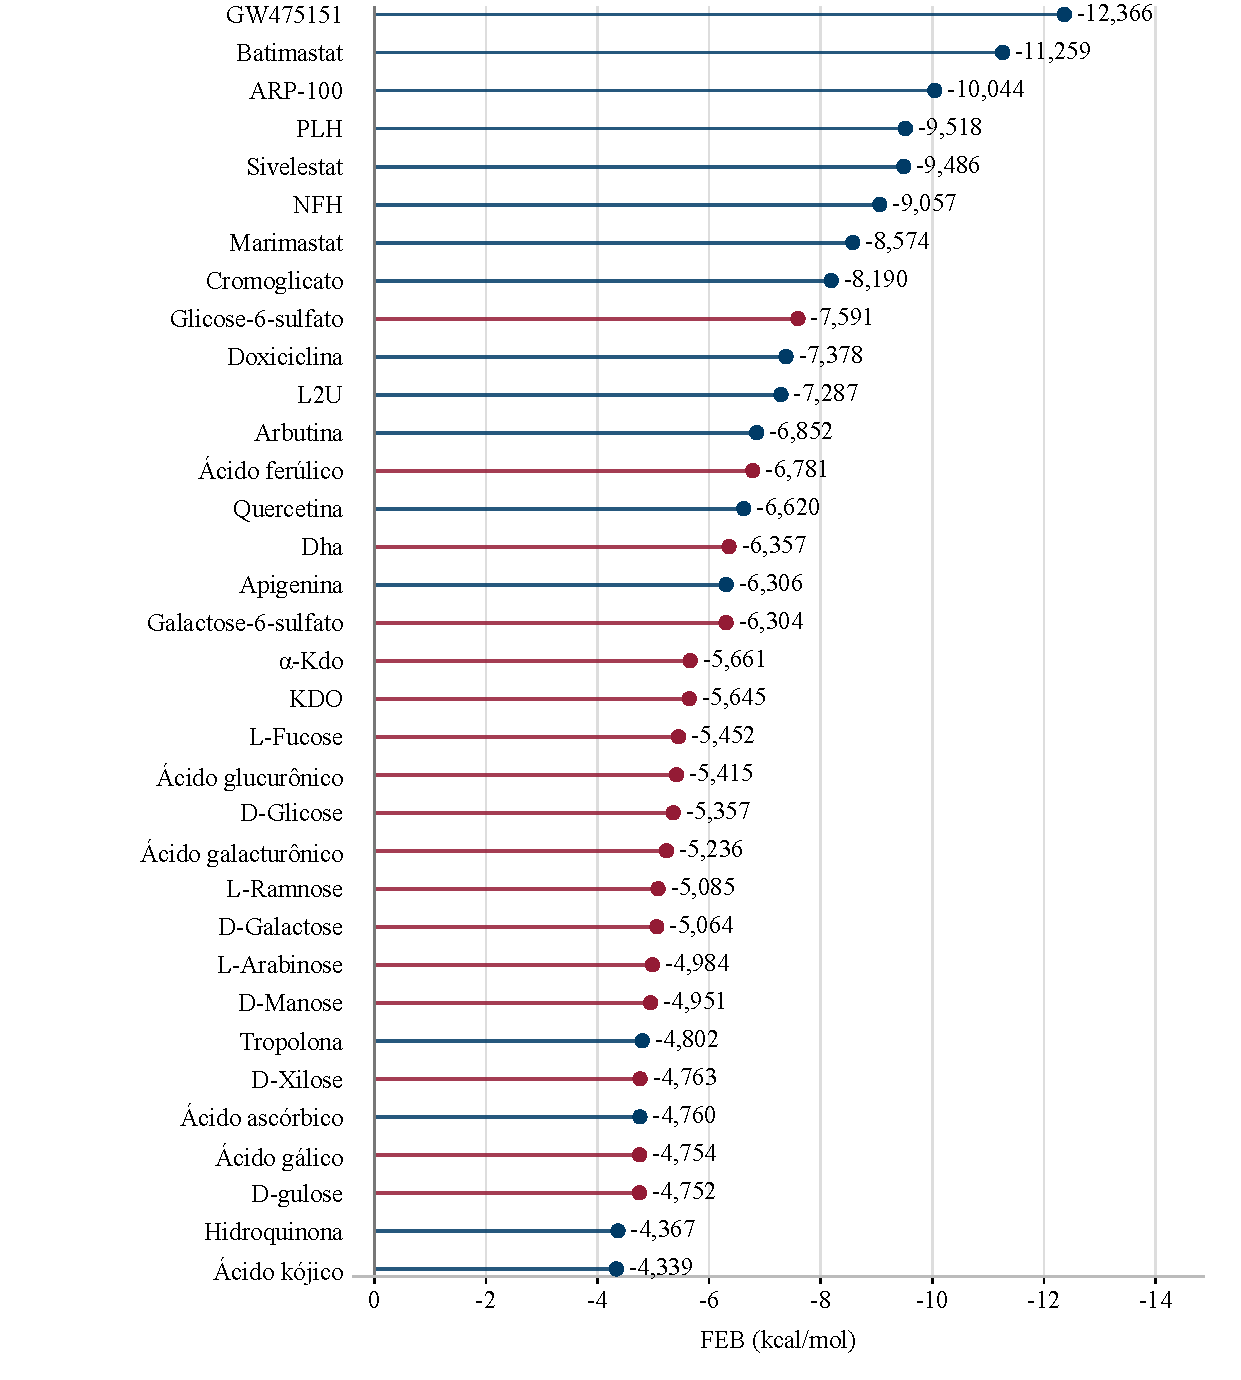
\includegraphics[width=\linewidth,height=17.5cm,keepaspectratio]{image/lollipop/lollipop_1HFC.pdf}
\end{figure}

A Figura~\ref{fig:lollipop_1HFC} mostra GW475151 (-12,366~kcal/mol) e batimastat (-11,259~kcal/mol) nas primeiras posições entre os ligantes comerciais e coocristalizados. No conjunto de prospecção, a glicose-6-sulfato (-7,591~kcal/mol) foi seguida por ácido ferúlico (-6,781~kcal/mol) e Dha (-6,357~kcal/mol). A glicose-6-sulfato ocupou a nona posição entre os 34 ligantes, com FEB 4,775~kcal/mol menos negativa que a de GW475151. Sua posição à frente de parte dos ligantes comerciais e coocristalizados a destaca para investigação posterior.

As medianas de FEB foram -7,378~kcal/mol para os ligantes comerciais e coocristalizados e -5,357~kcal/mol para os compostos em prospecção. A pontuação da glicose-6-sulfato foi mais negativa que a primeira mediana, o que a distingue dos demais compostos de prospecção avaliados em MMP-1. O resultado fundamenta sua seleção para estudos posteriores com MMP-1, nos quais sua interação e eventual efeito sobre a atividade enzimática deverão ser avaliados experimentalmente.


Na Figura~\ref{fig:mapa_interacoes_1HFC}, GLU~219 da cadeia A apresenta contato com 27 ligantes, seguido por LEU~181 e ALA~182, ambos com 25. O empate indica igual abrangência entre os ligantes, e não igual intensidade de interação. A presença desses resíduos em grande parte das poses evidencia um conjunto de resíduos frequentemente compartilhados pelas poses analisadas.

A distribuição por grupo destacou GLU~219, com contato em 12 ligantes comerciais e coocristalizados e 15 compostos em prospecção, e LEU~181, com contato em 12 e 13 ligantes, respectivamente; ambos pertencem à cadeia A. O conjunto de prospecção participou amplamente dos contatos mais recorrentes, apesar de apresentar mediana de FEB menos negativa. A glicose-6-sulfato interagiu com nove resíduos distintos, enquanto L2U alcançou dez sem liderar a classificação por FEB. Assim, a diversidade de resíduos contatados não determinou, por si só, a menor pontuação.

\begin{figure}[H]\centering
\caption[Matriz de contatos em MMP-1 (1HFC)]{Matriz de presença das interações dos 34 ligantes com os resíduos de MMP-1 (1HFC).}\label{fig:mapa_interacoes_1HFC}


\par\vspace{3pt}\begin{tabular}{@{}l@{\hspace{1em}}l@{\hspace{1em}}l@{}}\tikz[baseline=-.4ex]\filldraw[fill=mapacomercial,draw=black!40] (0,0) rectangle (.28,.28);\ Comerciais e coocristalizados & \tikz[baseline=-.4ex]\filldraw[fill=mapatetra,draw=black!40] (0,0) rectangle (.28,.28);\ Prospecção & \tikz[baseline=-.4ex]\filldraw[fill=white,draw=black!40] (0,0) rectangle (.28,.28);\ Sem contato registrado\end{tabular}\par\vspace{3pt}\normalsize X: contato presente; resíduos da cadeia A.\par\vspace{5pt}
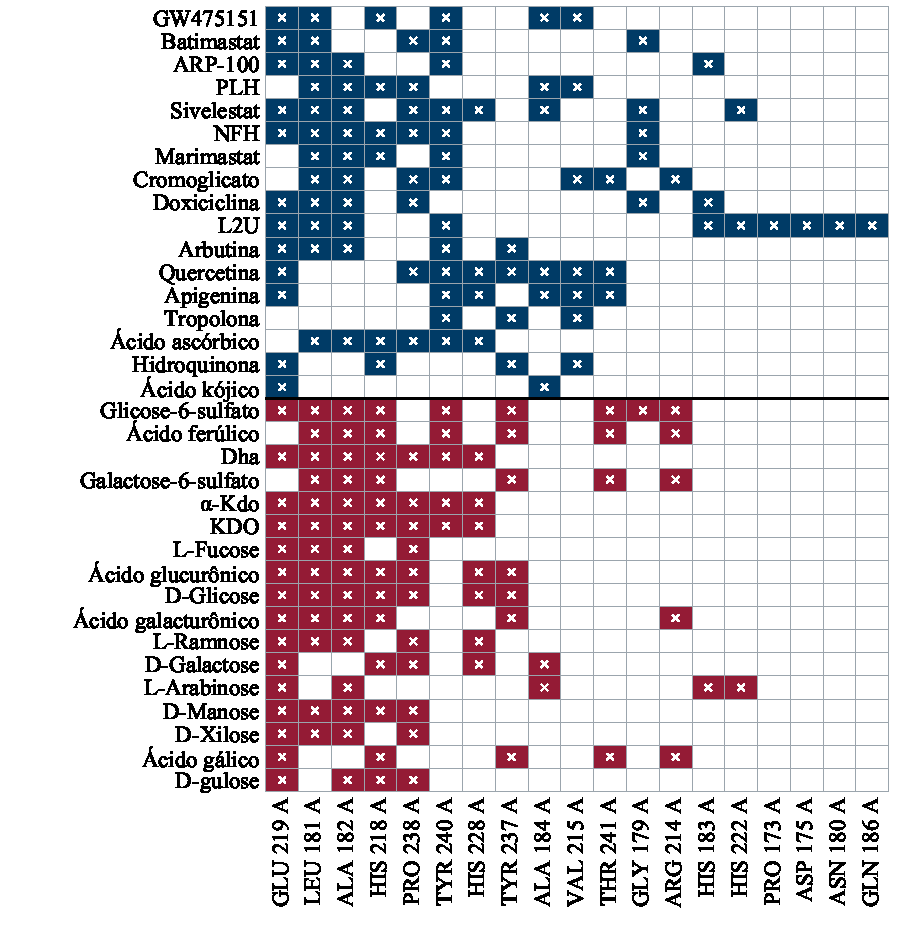
\includegraphics[width=15.2cm,height=14cm,keepaspectratio]{image/interacoes/mapa_interacoes_1HFC.pdf}

\fonte{Relatórios PLIP da matriz principal. Resíduos da cadeia A, ordenados pelo número decrescente de ligantes com interação; empates por número do resíduo.}
\end{figure}

Na comparação direta, GW475151 e glicose-6-sulfato compartilharam contatos com LEU~181, HIS~218, TYR~240 e GLU~219. A glicose-6-sulfato apresentou também contatos com GLY~179, ALA~182, THR~241, ARG~214 e TYR~237; GW475151 contatou ainda VAL~215 e ALA~184. A FEB da glicose-6-sulfato foi 4,775~kcal/mol menos negativa que a de GW475151.





\FloatBarrier
\subsubsection{Gelatinase A humana (MMP-2, 8H78)}
A figura de redocking mostra pose 04 de L2U, selecionada pela sobreposição conformacional, e não representa a pose 01 de menor FEB da matriz principal. As duas seleções atendem a critérios distintos e não devem ser interpretadas como uma única conformação \parencite{takeuchi2023,cole2005}.
O relatório de L2U foi recalculado sem TZ, enquanto o de galactose-6-sulfato corresponde ao relatório preservado da execução. Essa diferença de proveniência limita a comparação direta de suas contagens de interações.



\begin{figure}[H]
\centering
\caption[Docking em MMP-2 (8H78)]{Pontuações de docking (FEB, kcal/mol) dos 34 ligantes para a gelatinase A humana (MMP-2, 8H78).}\label{fig:lollipop_8H78}
\par\vspace{2pt}\begin{tabular}{@{}l@{\hspace{1.5em}}l@{}}\tikz[baseline=-.4ex]\filldraw[fill=mapacomercial,draw=black!40] (0,0) rectangle (.28,.28);\ Ligantes comerciais e coocristalizados & \tikz[baseline=-.4ex]\filldraw[fill=mapatetra,draw=black!40] (0,0) rectangle (.28,.28);\ Prospecção\end{tabular}\par\vspace{2pt}
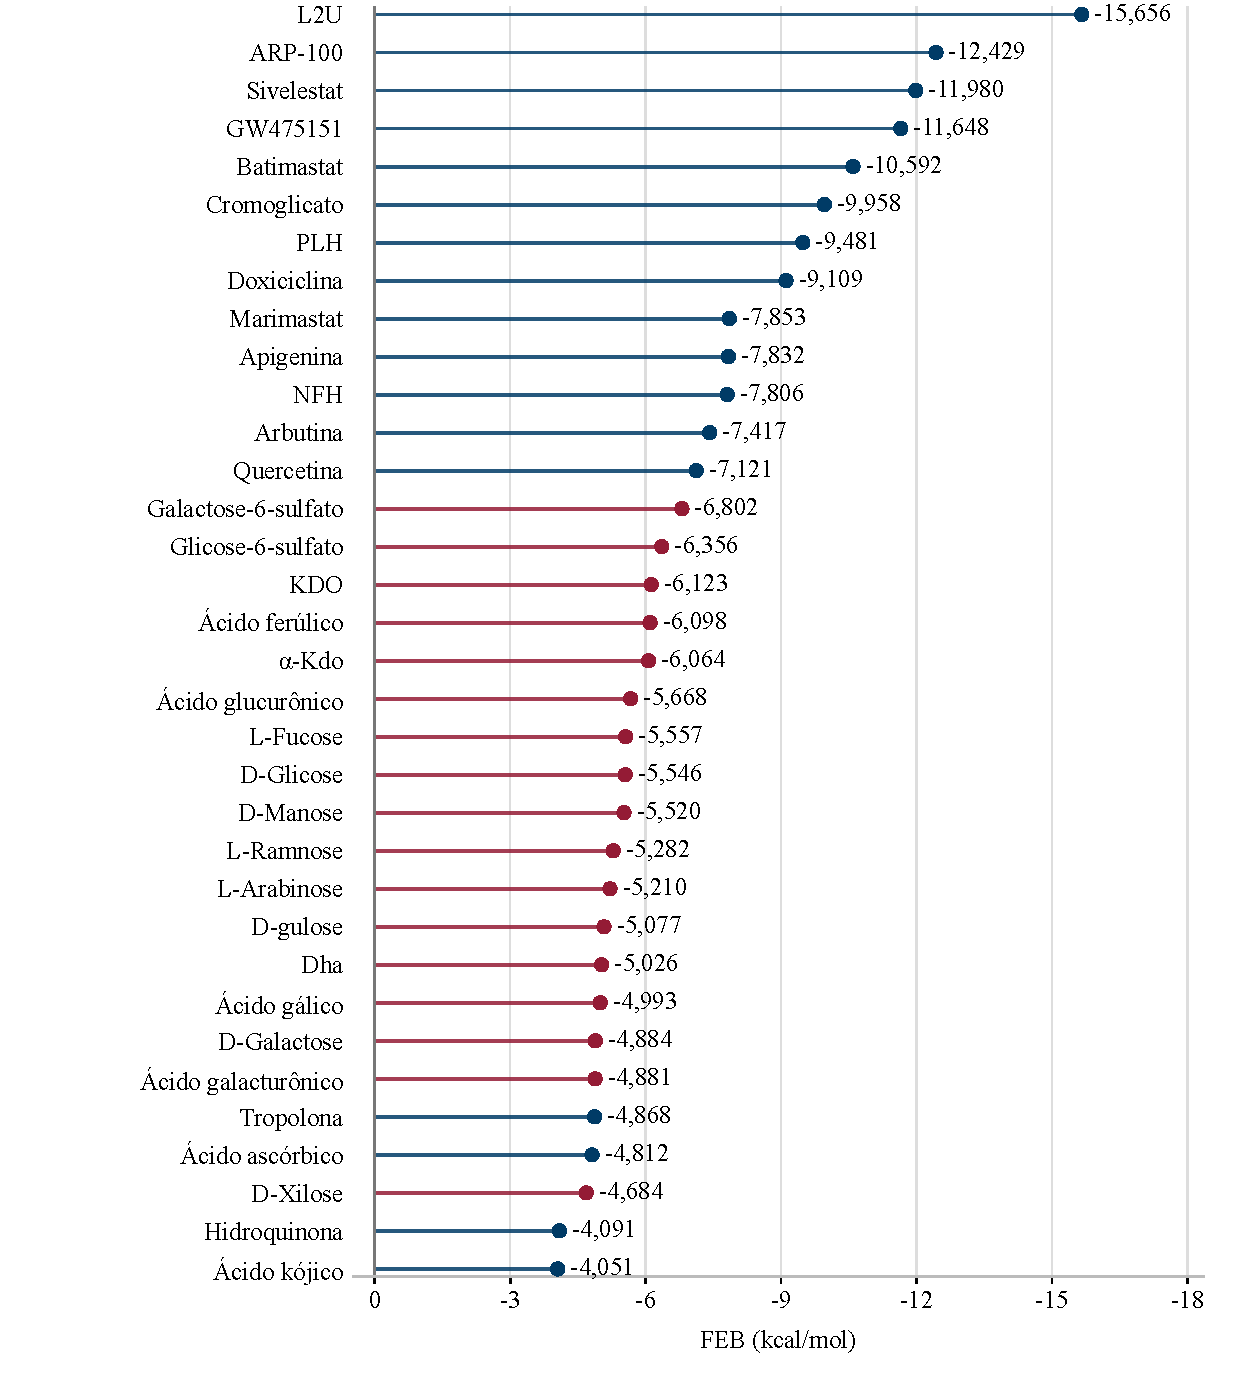
\includegraphics[width=\linewidth,height=17.5cm,keepaspectratio]{image/lollipop/lollipop_8H78.pdf}
\end{figure}

A Figura~\ref{fig:lollipop_8H78} mostra L2U (-15,656~kcal/mol) na primeira posição do conjunto de ligantes comerciais e coocristalizados, seguido por ARP-100 (-12,429~kcal/mol), com diferença de 3,227~kcal/mol. No conjunto de prospecção, destacaram-se galactose-6-sulfato (-6,802~kcal/mol), glicose-6-sulfato (-6,356~kcal/mol) e KDO (-6,123~kcal/mol). A galactose-6-sulfato ficou na 14ª posição geral, com FEB 8,854~kcal/mol menos negativa que a de L2U. Ela liderou o conjunto de prospecção e ficou abaixo dos primeiros colocados entre os ligantes comerciais e coocristalizados na classificação conjunta.

As medianas de FEB foram -7,853~kcal/mol para os ligantes comerciais e coocristalizados e -5,520~kcal/mol para o conjunto de prospecção. Além da distância entre L2U e o segundo colocado, a mediana comercial mais negativa mostra uma diferença entre os conjuntos. A recorrência de derivados sulfatados de açúcares entre os destaques das metaloproteinases orienta estudos posteriores com essas moléculas. A classificação, entretanto, não estabelece seletividade entre os alvos nem sua ocorrência na SPE de \textit{T. chuii}.


A Figura~\ref{fig:mapa_interacoes_8H78} destaca THR~144, ILE~142 e ALA~140 da cadeia A, com contatos em 27, 20 e 18 ligantes, respectivamente. As colunas mais recorrentes mostram resíduos compartilhados por diferentes compostos, enquanto os contatos menos frequentes distinguem parte das poses. A análise complementa a ordenação por FEB, sem substituir a avaliação energética.

A distribuição por grupo destacou THR~144 (10 comerciais e 17 compostos do conjunto de prospecção) e ILE~142 (8 comerciais e 12 compostos do conjunto de prospecção), ambos da cadeia A. Como THR~144 ocorreu nos contatos de todos os ligantes do conjunto de prospecção, esse resíduo não diferencia a liderança de galactose-6-sulfato e glicose-6-sulfato. L2U apresentou contatos com 15 resíduos distintos, mas essa observação isolada não estabelece uma relação geral entre quantidade de contatos e FEB.

\begin{figure}[H]\centering
\caption[Matriz de contatos em MMP-2 (8H78)]{Matriz de presença das interações dos 34 ligantes com os resíduos da gelatinase A humana (MMP-2, 8H78).}\label{fig:mapa_interacoes_8H78}
\par\vspace{3pt}\begin{tabular}{@{}l@{\hspace{1em}}l@{\hspace{1em}}l@{}}\tikz[baseline=-.4ex]\filldraw[fill=mapacomercial,draw=black!40] (0,0) rectangle (.28,.28);\ Comerciais e coocristalizados & \tikz[baseline=-.4ex]\filldraw[fill=mapatetra,draw=black!40] (0,0) rectangle (.28,.28);\ Prospecção & \tikz[baseline=-.4ex]\filldraw[fill=white,draw=black!40] (0,0) rectangle (.28,.28);\ Sem contato registrado\end{tabular}\par\vspace{3pt}\normalsize X: contato presente; resíduos da cadeia A.\par\vspace{5pt}
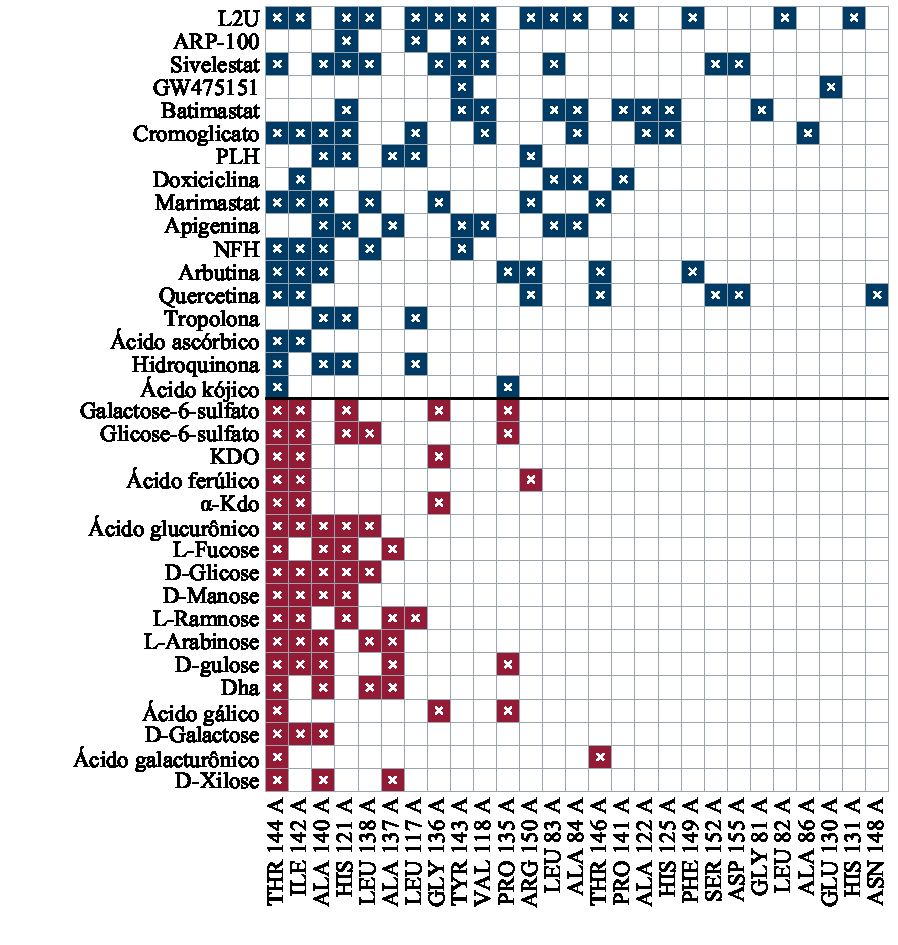
\includegraphics[width=15.2cm,height=14cm,keepaspectratio]{image/interacoes/mapa_interacoes_8H78.pdf}
\end{figure}

Na comparação direta, L2U e galactose-6-sulfato compartilharam contatos com GLY~136, HIS~121, ILE~142 e THR~144. L2U apresentou outros onze resíduos de contato, enquanto a galactose-6-sulfato também contatou PRO~135. A FEB da galactose-6-sulfato foi 8,854~kcal/mol menos negativa que a de L2U.







\FloatBarrier
\FloatBarrier
\subsubsection{Proteína humana relacionada à tirosinase 1 (TYRP1, 5M8P)}
A análise de 5M8P corresponde à TYRP1 humana, que apresenta centro binuclear de zinco. A L-tirosina foi examinada separadamente como referência estrutural. A classificação dos 34 ligantes e seus contatos são discutidos para TYRP1 humana; eles não demonstram inibição enzimática nem efeito despigmentante \parencite{lai2017}.
A análise conjunta dos gráficos e dos mapas permite comparar a pontuação de batimastat e ácido ferúlico com a distribuição de seus contatos no receptor.



\begin{figure}[H]
\centering
\caption[Docking em TYRP1 (5M8P)]{Pontuações de docking (FEB, kcal/mol) dos 34 ligantes para a TYRP1 humana (5M8P).}\label{fig:lollipop_5M8P}
\par\vspace{2pt}\begin{tabular}{@{}l@{\hspace{1.5em}}l@{}}\tikz[baseline=-.4ex]\filldraw[fill=mapacomercial,draw=black!40] (0,0) rectangle (.28,.28);\ Ligantes comerciais e coocristalizados & \tikz[baseline=-.4ex]\filldraw[fill=mapatetra,draw=black!40] (0,0) rectangle (.28,.28);\ Prospecção\end{tabular}\par\vspace{2pt}
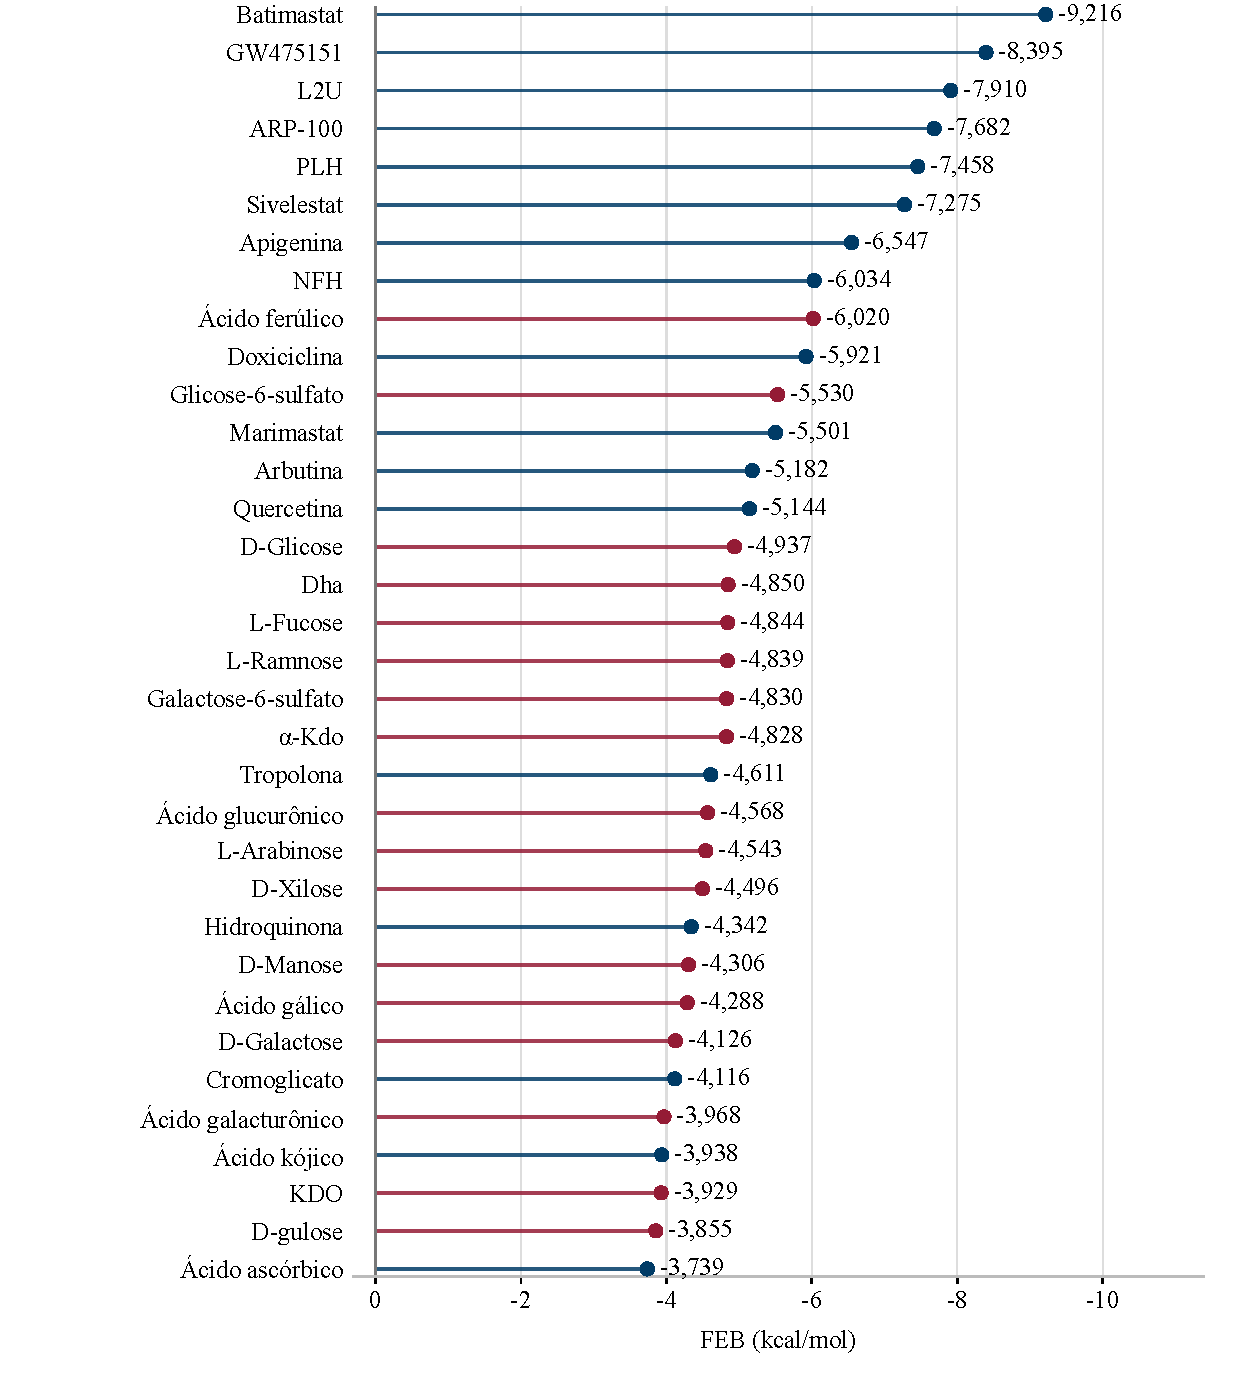
\includegraphics[width=\linewidth,height=17.5cm,keepaspectratio]{image/lollipop/lollipop_5M8P.pdf}
\end{figure}

Na Figura~\ref{fig:lollipop_5M8P}, batimastat (-9,216~kcal/mol) e GW475151 (-8,395~kcal/mol) ocupam as primeiras posições entre os 17 ligantes comerciais e coocristalizados. No conjunto de prospecção, ácido ferúlico (-6,020~kcal/mol), glicose-6-sulfato (-5,530~kcal/mol) e D-glicose (-4,937~kcal/mol) apresentaram as menores FEB. O ácido ferúlico ficou na nona posição geral, com pontuação 3,196~kcal/mol menos negativa que a de batimastat. A L-tirosina suplementar não integra essa classificação.

As medianas de FEB foram -5,921~kcal/mol para os ligantes comerciais e coocristalizados e -4,568~kcal/mol para os compostos em prospecção. A pontuação do ácido ferúlico foi ligeiramente mais negativa que a primeira mediana, embora permaneça distante dos líderes do conjunto. Esse resultado o diferencia dos demais compostos de seu grupo. Os ligantes comerciais e coocristalizados selecionados incluem moléculas estudadas para outros alvos; em TYRP1, suas pontuações permitem comparar as poses previstas nesse receptor.


Na Figura~\ref{fig:mapa_interacoes_5M8P}, ASP~212, GLU~216 e THR~391 da cadeia A apresentam contatos com 12, 11 e 10 ligantes, respectivamente. O mapa distribui as presenças por 60 resíduos, com numerosas colunas de baixa recorrência. Esse padrão indica maior diversidade de resíduos envolvidos entre as poses apresentadas, sem demonstrar seletividade ou inibição de TYRP1.

A distribuição por grupo destacou ASP~212, com contato em 10 ligantes comerciais e coocristalizados e 2 compostos em prospecção, e GLU~216, com contato em 9 e 2 ligantes, respectivamente; ambos pertencem à cadeia A. Os contatos mais recorrentes vieram principalmente do conjunto comercial e coocristalizado. Além disso, 28 dos 60 resíduos apareceram em apenas um ligante. Essa dispersão motiva verificar a localização e a orientação das poses antes de atribuir relevância funcional aos contatos menos recorrentes. O número total de resíduos contatados no conjunto não mede a estabilidade dos complexos.

\begin{landscape}

\begin{figure}[H]\centering
\caption[Matriz de contatos em TYRP1 (5M8P)]{Matriz de presença das interações dos 34 ligantes com os resíduos da TYRP1 humana (5M8P).}\label{fig:mapa_interacoes_5M8P}
\par\vspace{3pt}\begin{tabular}{@{}l@{\hspace{1em}}l@{\hspace{1em}}l@{}}\tikz[baseline=-.4ex]\filldraw[fill=mapacomercial,draw=black!40] (0,0) rectangle (.28,.28);\ Comerciais e coocristalizados & \tikz[baseline=-.4ex]\filldraw[fill=mapatetra,draw=black!40] (0,0) rectangle (.28,.28);\ Prospecção & \tikz[baseline=-.4ex]\filldraw[fill=white,draw=black!40] (0,0) rectangle (.28,.28);\ Sem contato registrado\end{tabular}\par\vspace{3pt}\normalsize X: contato presente; resíduos da cadeia A.\par\vspace{5pt}
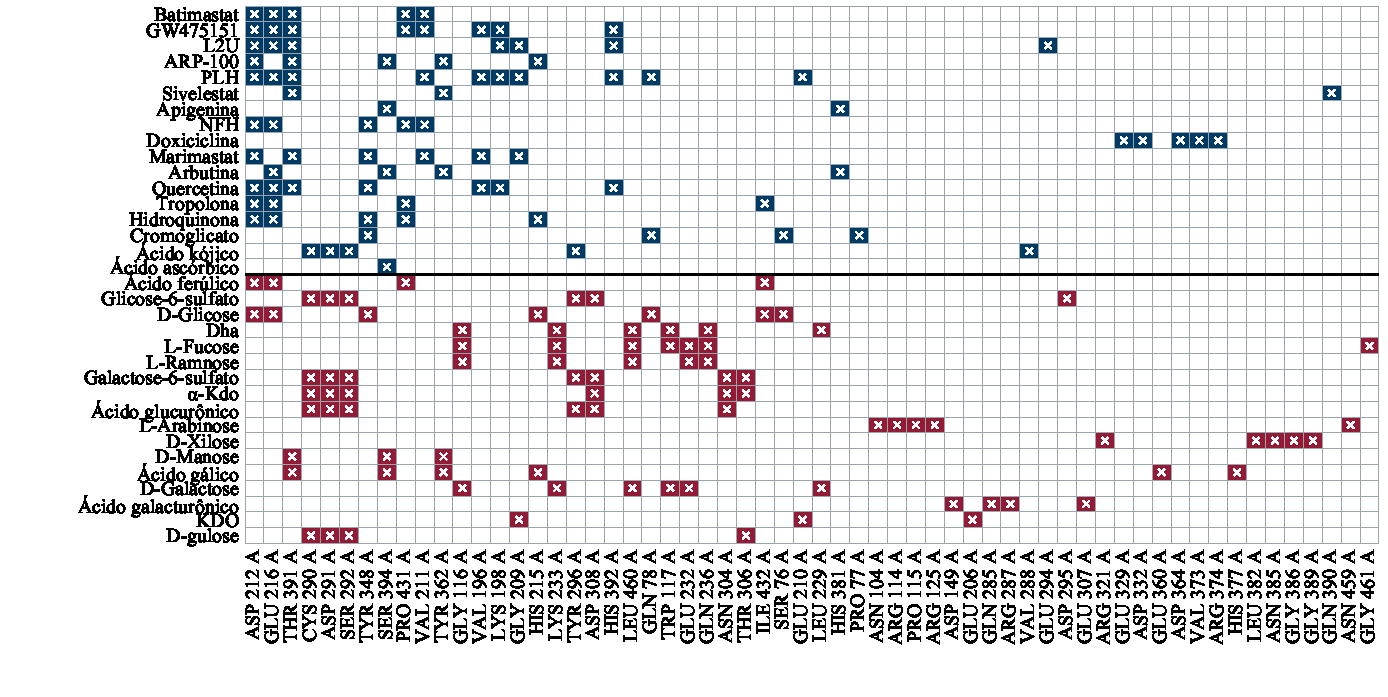
\includegraphics[width=23.5cm,height=11.8cm,keepaspectratio]{image/interacoes/mapa_interacoes_5M8P.pdf}
\end{figure}

\end{landscape}

Na comparação direta, batimastat e ácido ferúlico compartilharam contatos com ASP~212, GLU~216 e PRO~431. Batimastat também contatou THR~391 e VAL~211, enquanto o ácido ferúlico contatou ILE~432. A FEB do ácido ferúlico foi 3,196~kcal/mol menos negativa que a de batimastat.











\FloatBarrier
\subsubsection{Elastase de neutrófilos humanos (1H1B)}
Os resultados de elastase incorporam as coordenadas corrigidas para os dois grupos. A sobreposição de GW475151 apresentada na subseção de RMSD pertence à execução anterior e não caracteriza as novas poses. A análise a seguir combina a classificação por FEB com os contatos identificados nas poses selecionadas \parencite{macdonald2002,cole2005,warren2006}.

A Figura~\ref{fig:lollipop_1H1B} apresenta a classificação conjunta dos ligantes, mantendo a distinção entre os grupos.

\begin{figure}[H]
\centering
\caption[Docking em elastase (1H1B)]{Pontuações de docking (FEB, kcal/mol) dos 34 ligantes para a elastase de neutrófilos humanos (1H1B).}\label{fig:lollipop_1H1B}
\par\vspace{2pt}\begin{tabular}{@{}l@{\hspace{1.5em}}l@{}}\tikz[baseline=-.4ex]\filldraw[fill=mapacomercial,draw=black!40] (0,0) rectangle (.28,.28);\ Ligantes comerciais e coocristalizados & \tikz[baseline=-.4ex]\filldraw[fill=mapatetra,draw=black!40] (0,0) rectangle (.28,.28);\ Prospecção\end{tabular}\par\vspace{2pt}
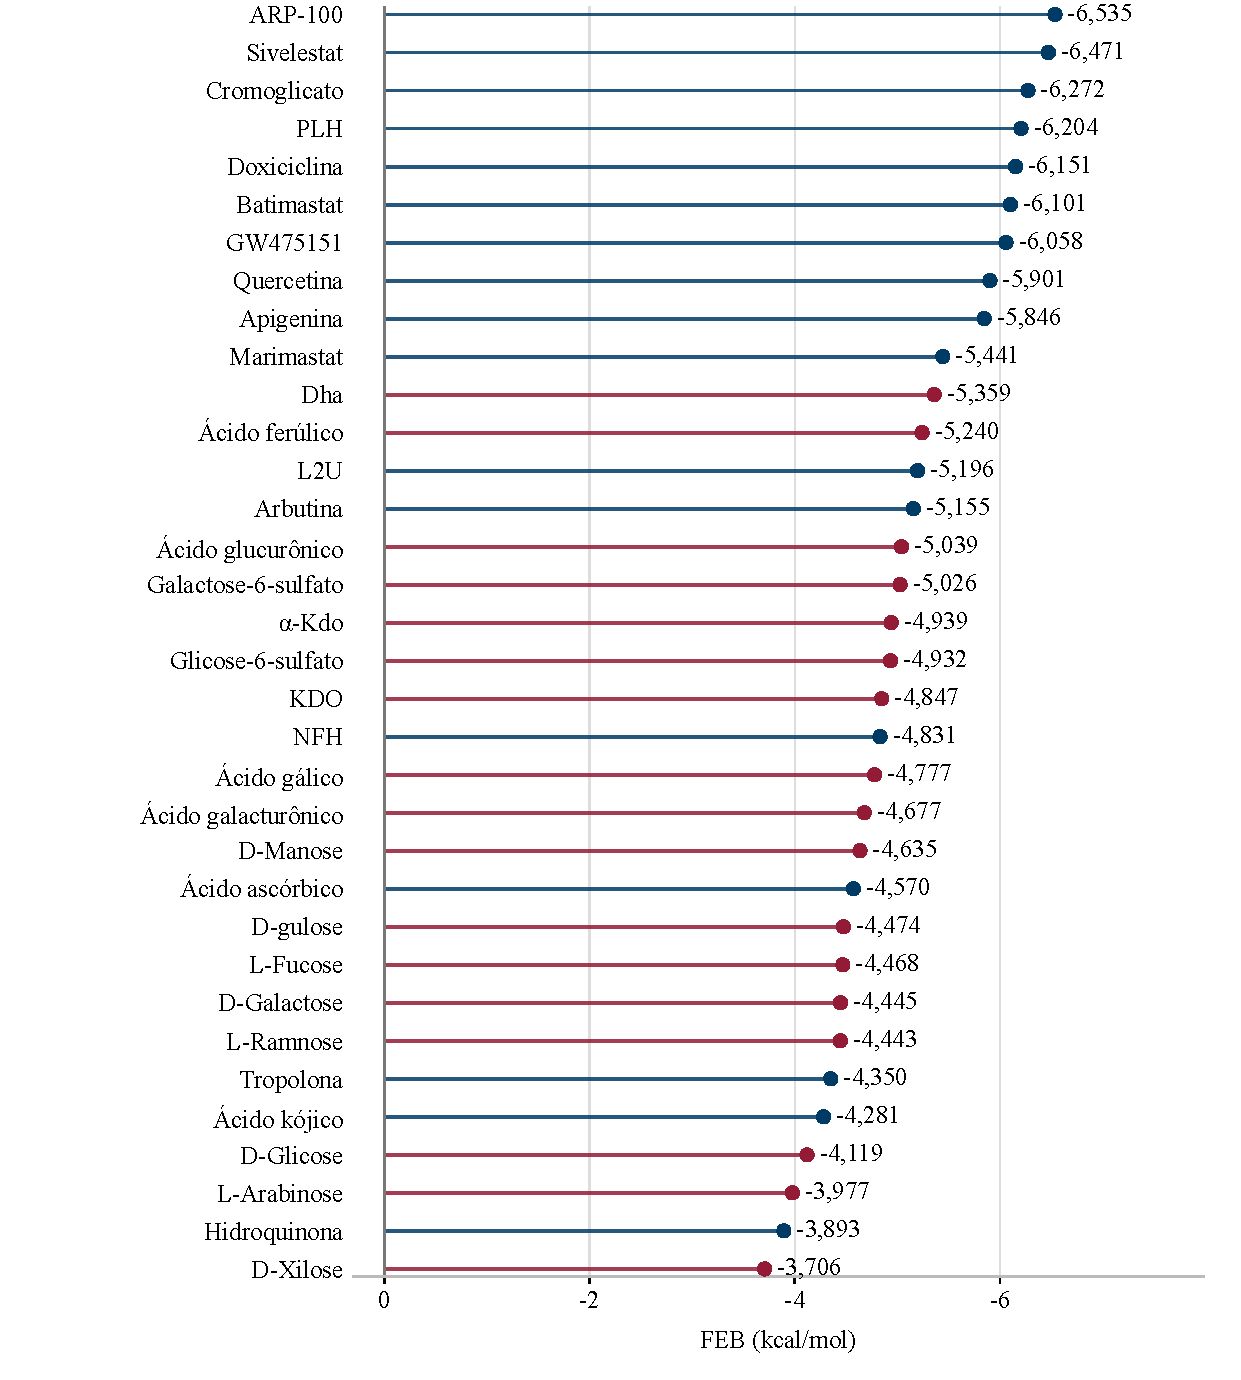
\includegraphics[width=\linewidth,height=17.5cm,keepaspectratio]{image/lollipop/lollipop_1H1B.pdf}
\end{figure}

Na execução atualizada, ARP-100 (-6,535~kcal/mol) e Sivelestat (-6,471~kcal/mol) ocuparam as duas primeiras posições entre os ligantes comerciais e coocristalizados, com diferença de 0,064~kcal/mol. No conjunto de prospecção, destacaram-se Dha (-5,359~kcal/mol), ácido ferúlico (-5,240~kcal/mol) e ácido glucurônico (-5,039~kcal/mol). Dha ocupou a 11ª posição entre os 34 ligantes, com FEB 1,176~kcal/mol menos negativa que a do primeiro colocado do conjunto comercial e coocristalizado.

As medianas foram -5,846~kcal/mol para os ligantes comerciais e coocristalizados e -4,677~kcal/mol para o conjunto de prospecção. As faixas de FEB foram de -6,535 a -3,893~kcal/mol e de -5,359 a -3,706~kcal/mol, respectivamente. Houve sobreposição entre as faixas: os melhores compostos do conjunto de prospecção apresentaram pontuações mais negativas que parte dos ligantes comerciais e coocristalizados, embora não alcançassem o líder. A sobreposição descreve o posicionamento relativo dos ligantes nesta triagem, sem indicar equivalência de atividade biológica entre os grupos.

A Figura~\ref{fig:mapa_interacoes_1H1B} foi regenerada com os relatórios PLIP das mesmas poses de menor FEB utilizadas na classificação. VAL~216 (cadeia A) apresentou contato com 23 ligantes; SER~195 (cadeia A) apresentou contato com 21 ligantes; HIS~57 (cadeia A) apresentou contato com 14 ligantes. O mapa reúne 19 resíduos distintos.

A distribuição por grupo mostrou VAL~216 em 11 ligantes comerciais e coocristalizados e 12 compostos em prospecção; SER~195 ocorreu em 7 e 14 ligantes, respectivamente. ARP-100 apresentou contatos com 6 resíduos distintos, e Dha, com 5. Cada par ligante--resíduo foi contado uma única vez. A maior recorrência de SER~195 no conjunto de prospecção, em conjunto com sua mediana de FEB menos negativa, reforça que presença de contato e classificação energética descrevem aspectos diferentes das poses.

\begin{figure}[H]\centering
\caption[Matriz de contatos em elastase (1H1B)]{Matriz de presença das interações dos 34 ligantes com os resíduos de elastase de neutrófilos humanos (1H1B).}\label{fig:mapa_interacoes_1H1B}


\par\vspace{3pt}\begin{tabular}{@{}l@{\hspace{1em}}l@{\hspace{1em}}l@{}}\tikz[baseline=-.4ex]\filldraw[fill=mapacomercial,draw=black!40] (0,0) rectangle (.28,.28);\ Comerciais e coocristalizados & \tikz[baseline=-.4ex]\filldraw[fill=mapatetra,draw=black!40] (0,0) rectangle (.28,.28);\ Prospecção & \tikz[baseline=-.4ex]\filldraw[fill=white,draw=black!40] (0,0) rectangle (.28,.28);\ Sem contato registrado\end{tabular}\par\vspace{3pt}\normalsize X: contato presente; resíduos identificados por aminoácido, número e cadeia.\par\vspace{5pt}
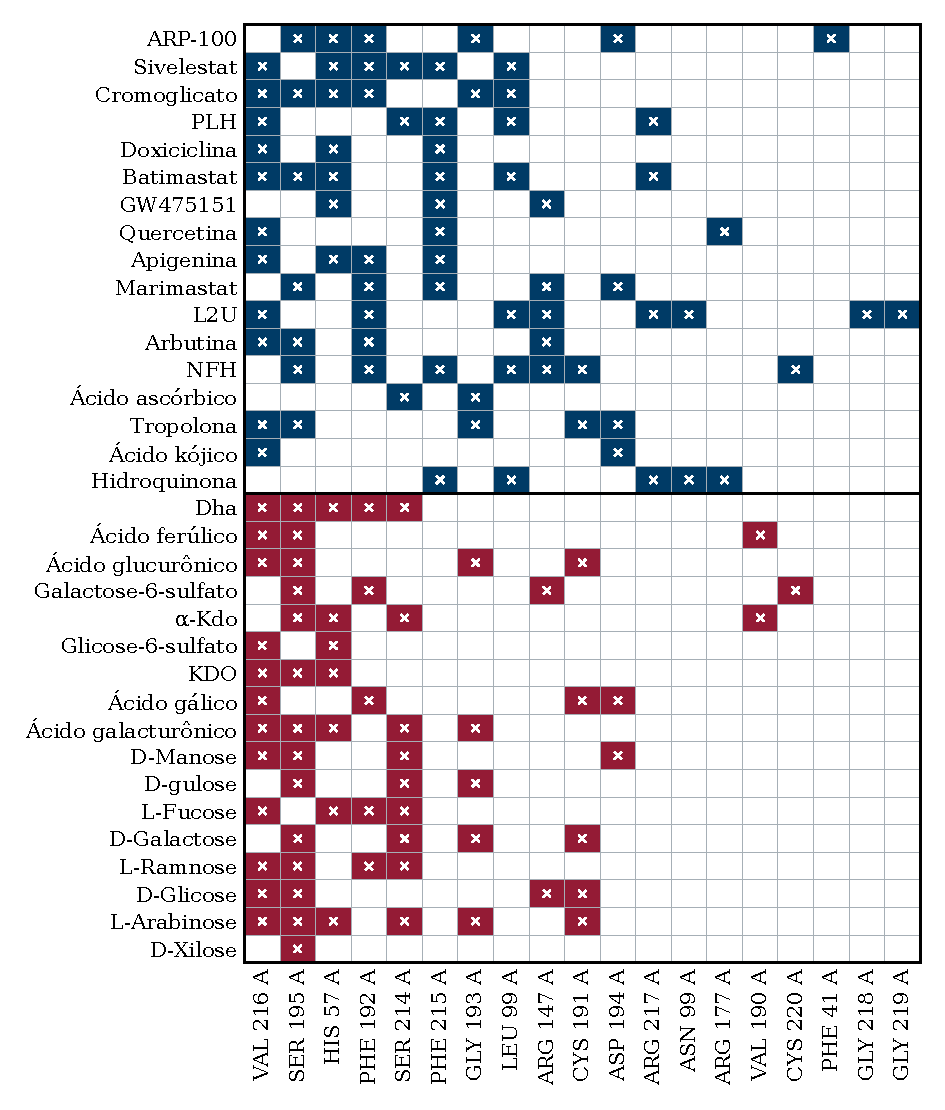
\includegraphics[width=15.2cm,height=14cm,keepaspectratio]{image/interacoes/mapa_interacoes_1H1B.pdf}

\fonte{PLIP das poses de menor FEB da execução corrigida; resíduos em ordem decrescente de recorrência.}
\end{figure}

Na comparação direta, ARP-100 e Dha compartilharam contatos com HIS~57, PHE~192 e SER~195. ARP-100 também contatou ASP~194, GLY~193 e PHE~41; Dha apresentou contatos adicionais com SER~214 e VAL~216. A FEB de Dha foi 1,176~kcal/mol menos negativa que a de ARP-100.

\FloatBarrier
\subsubsection{Hialuronidase humana 1 (2PE4)}
A execução com coordenadas corrigidas substitui os valores anteriores dos dois grupos. A ausência de um inibidor cristalográfico equivalente impede a avaliação de redocking por essa referência; nenhum RMSD foi atribuído a 2PE4 \parencite{chao2007,cole2005}.

A Figura~\ref{fig:lollipop_2PE4} apresenta a classificação conjunta dos ligantes, mantendo a distinção entre os grupos.

\begin{figure}[H]
\centering
\caption[Docking em hialuronidase 1 (2PE4)]{Pontuações de docking (FEB, kcal/mol) dos 34 ligantes para a hialuronidase humana 1 (2PE4).}\label{fig:lollipop_2PE4}
\par\vspace{2pt}\begin{tabular}{@{}l@{\hspace{1.5em}}l@{}}\tikz[baseline=-.4ex]\filldraw[fill=mapacomercial,draw=black!40] (0,0) rectangle (.28,.28);\ Ligantes comerciais e coocristalizados & \tikz[baseline=-.4ex]\filldraw[fill=mapatetra,draw=black!40] (0,0) rectangle (.28,.28);\ Prospecção\end{tabular}\par\vspace{2pt}
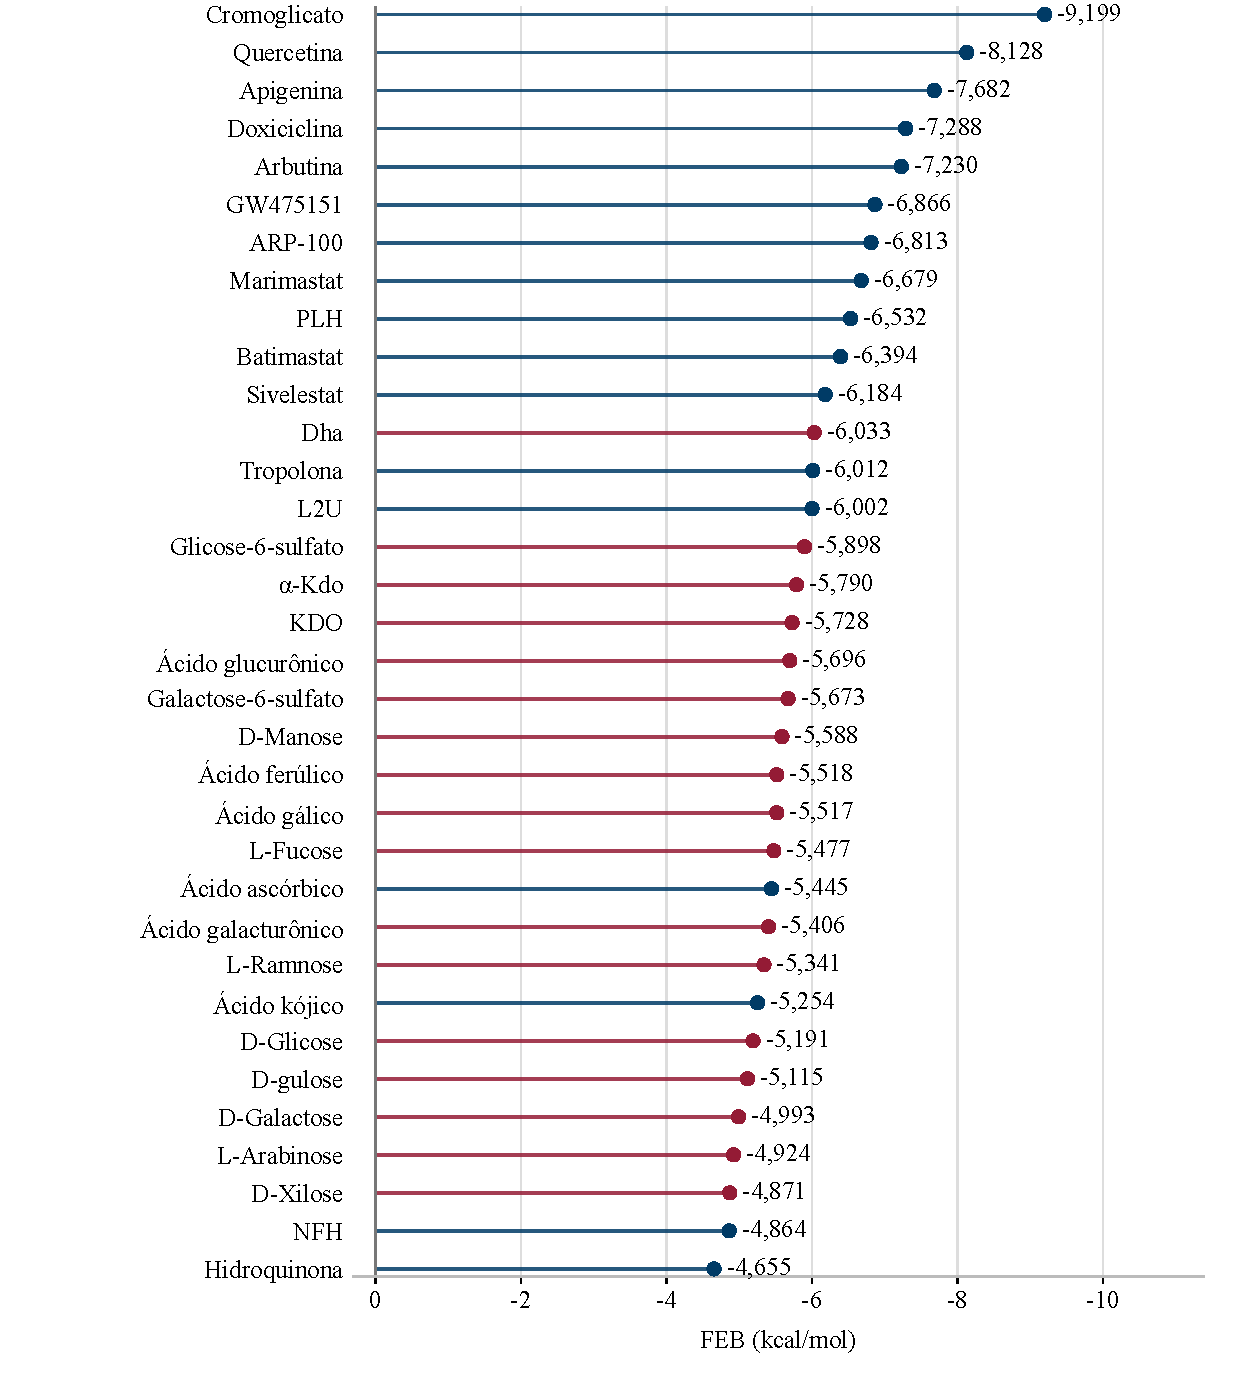
\includegraphics[width=\linewidth,height=17.5cm,keepaspectratio]{image/lollipop/lollipop_2PE4.pdf}
\end{figure}

Na execução atualizada, cromoglicato (-9,199~kcal/mol) e quercetina (-8,128~kcal/mol) ocuparam as primeiras posições entre os ligantes comerciais e coocristalizados, com diferença de 1,071~kcal/mol. No conjunto de prospecção, destacaram-se Dha (-6,033~kcal/mol), glicose-6-sulfato (-5,898~kcal/mol) e $\alpha$-Kdo (-5,790~kcal/mol). Dha ocupou a 12ª posição entre os 34 ligantes, com FEB 3,166~kcal/mol menos negativa que a do primeiro colocado do conjunto comercial e coocristalizado.

As medianas foram -6,532~kcal/mol para os ligantes comerciais e coocristalizados e -5,517~kcal/mol para o conjunto de prospecção. As faixas de FEB foram de -9,199 a -4,655~kcal/mol e de -6,033 a -4,871~kcal/mol, respectivamente. Houve sobreposição entre as faixas: os melhores compostos do conjunto de prospecção apresentaram pontuações mais negativas que parte dos ligantes comerciais e coocristalizados, embora não alcançassem o líder. A sobreposição descreve o posicionamento relativo dos ligantes nesta triagem, sem indicar equivalência de atividade biológica entre os grupos.

A Figura~\ref{fig:mapa_interacoes_2PE4} foi regenerada com os relatórios PLIP das mesmas poses de menor FEB utilizadas na classificação. ARG~265 (cadeia A) apresentou contato com 14 ligantes; TYR~202 (cadeia A) apresentou contato com 13 ligantes; TYR~247 (cadeia A) apresentou contato com 13 ligantes. O mapa reúne 54 resíduos distintos.

A distribuição por grupo mostrou ARG~265 em 4 ligantes comerciais e coocristalizados e 10 compostos em prospecção; TYR~202 ocorreu em 7 e 6 ligantes, respectivamente. O cromoglicato apresentou contatos com 9 resíduos distintos, e Dha, com 8. Cada par ligante--resíduo foi contado uma única vez. A maior recorrência de ARG~265 no conjunto de prospecção caracteriza a distribuição das poses desse conjunto, sem explicar isoladamente sua classificação por FEB.

\begin{landscape}
\begin{figure}[H]\centering
\caption[Matriz de contatos em hialuronidase 1 (2PE4)]{Matriz de presença das interações dos 34 ligantes com os resíduos de hialuronidase humana 1 (2PE4).}\label{fig:mapa_interacoes_2PE4}


\par\vspace{3pt}\begin{tabular}{@{}l@{\hspace{1em}}l@{\hspace{1em}}l@{}}\tikz[baseline=-.4ex]\filldraw[fill=mapacomercial,draw=black!40] (0,0) rectangle (.28,.28);\ Comerciais e coocristalizados & \tikz[baseline=-.4ex]\filldraw[fill=mapatetra,draw=black!40] (0,0) rectangle (.28,.28);\ Prospecção & \tikz[baseline=-.4ex]\filldraw[fill=white,draw=black!40] (0,0) rectangle (.28,.28);\ Sem contato registrado\end{tabular}\par\vspace{3pt}\normalsize X: contato presente; resíduos identificados por aminoácido, número e cadeia.\par\vspace{5pt}
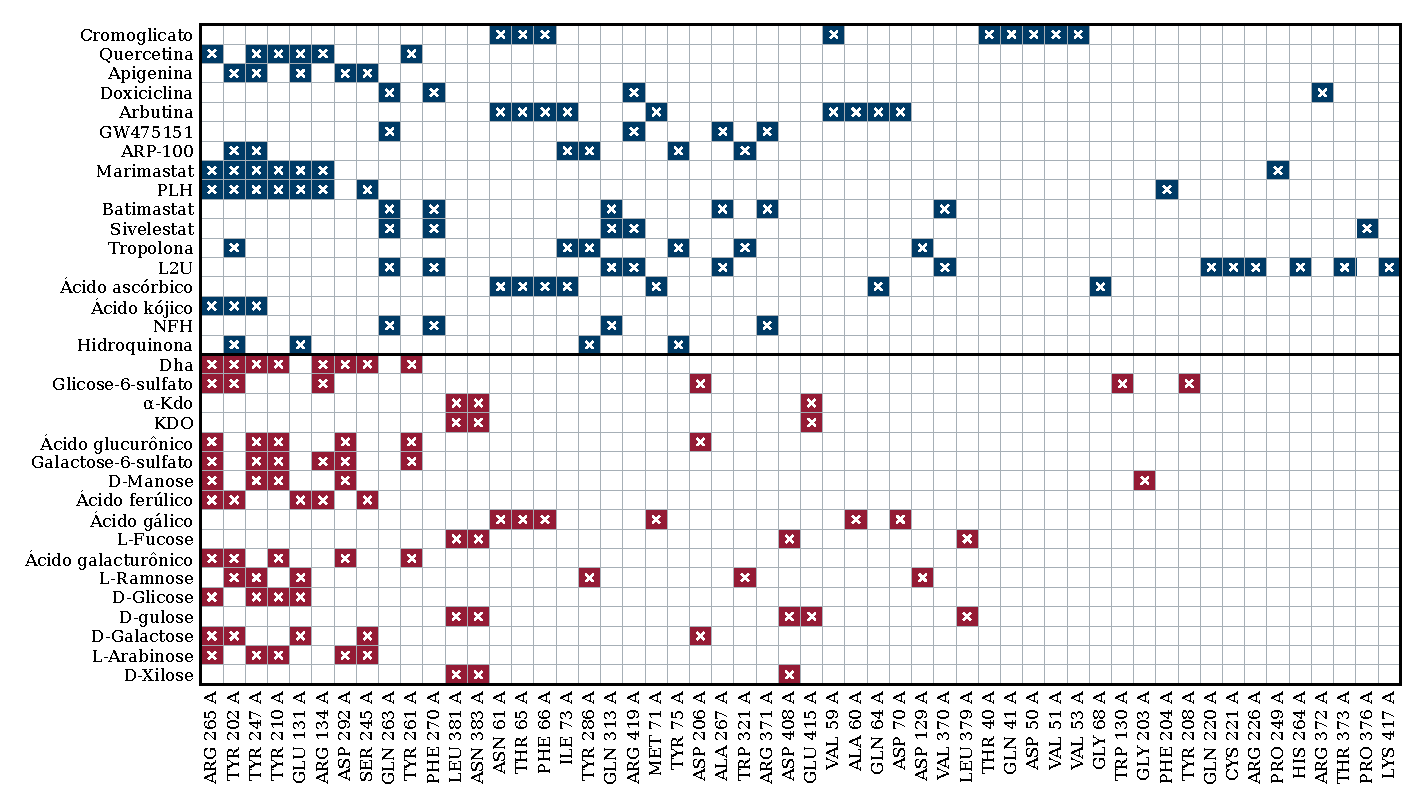
\includegraphics[width=23.5cm,height=12.3cm,keepaspectratio]{image/interacoes/mapa_interacoes_2PE4.pdf}

\fonte{PLIP das poses de menor FEB da execução corrigida; resíduos em ordem decrescente de recorrência.}
\end{figure}
\end{landscape}

Embora Dha tenha apresentado a menor FEB entre os compostos para prospecção em 2PE4, o ácido gálico foi selecionado para a comparação por compartilhar o maior número de resíduos com cromoglicato. Os dois ligantes compartilharam contatos com ASN~61, PHE~66 e THR~65. Cromoglicato também contatou ASP~50, GLN~41, THR~40, VAL~51, VAL~53 e VAL~59; o ácido gálico apresentou contatos adicionais com ALA~60, ASP~70 e MET~71. A FEB do ácido gálico foi 3,682~kcal/mol menos negativa que a de cromoglicato.

\FloatBarrier
\subsection{Síntese comparativa dos ligantes selecionados}
A Tabela~\ref{tab:sintese_pares} reúne, para cada receptor, o ligante de menor FEB do conjunto comercial e coocristalizado e o composto para prospecção selecionado pela sobreposição de contatos. Nos empates de sobreposição, a FEB mais negativa definiu a escolha. A coluna $n$ indica quantos resíduos distintos aparecem como contato nas duas poses; cada resíduo é contado uma vez por ligante. Os resíduos listados foram identificados pelo PLIP.

\begin{table}[H]
\centering
\caption[Síntese dos ligantes comparados por receptor]{Ligantes selecionados e resíduos compartilhados nas poses de docking.}
\label{tab:sintese_pares}
{\small\setlength{\tabcolsep}{4pt}
\begin{tabular}{C{0.9cm}C{3.0cm}C{3.0cm}C{1.0cm}C{6.2cm}}
\toprule
PDB & Ligante comparador (FEB, kcal/mol) & Composto para prospecção (FEB, kcal/mol) & n & Resíduos compartilhados \\
\midrule
1GKC & \shortstack{L2U\\($-13{,}465$)} & \shortstack{Glicose-6-sulfato\\($-6{,}971$)} & 5 & PRO~421, TYR~423, LEU~188, ALA~189, GLU~402 \\
1HFC & \shortstack{GW475151\\($-12{,}366$)} & \shortstack{Glicose-6-sulfato\\($-7{,}591$)} & 4 & LEU~181, HIS~218, TYR~240, GLU~219 \\
8H78 & \shortstack{L2U\\($-15{,}656$)} & \shortstack{Galactose-6-sulfato\\($-6{,}802$)} & 4 & GLY~136, HIS~121, ILE~142, THR~144 \\
5M8P & \shortstack{Batimastat\\($-9{,}216$)} & \shortstack{Ácido ferúlico\\($-6{,}020$)} & 3 & ASP~212, GLU~216, PRO~431 \\
1H1B & \shortstack{ARP-100\\($-6{,}535$)} & \shortstack{Dha\\($-5{,}359$)} & 3 & HIS~57, PHE~192, SER~195 \\
2PE4 & \shortstack{Cromoglicato\\($-9{,}199$)} & \shortstack{Ácido gálico\\($-5{,}517$)} & 3 & ASN~61, PHE~66, THR~65 \\
\bottomrule
\end{tabular}
}
\end{table}

Cada par apresentou de três a cinco resíduos de contato em comum. A glicose-6-sulfato compartilhou cinco resíduos com L2U em MMP-9 e quatro com GW475151 em MMP-1; nos demais receptores, os pares compartilharam três ou quatro resíduos. Em todos os casos, a FEB do ligante comercial ou coocristalizado foi mais negativa. As subseções por receptor também descrevem os resíduos exclusivos de cada pose, que ajudam a caracterizar as diferenças nos contatos previstos.

